% -*- Mode:TeX -*-

%% IMPORTANT: The official thesis specifications are available at:
%%            http://libraries.mit.edu/archives/thesis-specs/
%%
%%            Please verify your thesis' formatting and copyright
%%            assignment before submission.  If you notice any
%%            discrepancies between these templates and the 
%%            MIT Libraries' specs, please let us know
%%            by e-mailing thesis@mit.edu

%% The documentclass options along with the pagestyle can be used to generate
%% a technical report, a draft copy, or a regular thesis.  You may need to
%% re-specify the pagestyle after you \include  cover.tex.  For more
%% information, see the first few lines of mitthesis.cls. 

%\documentclass[12pt,vi,twoside]{mitthesis}
%%
%%  If you want your thesis copyright to you instead of MIT, use the
%%  ``vi'' option, as above.
%%
%\documentclass[12pt,twoside,leftblank]{mitthesis}
%%
%% If you want blank pages before new chapters to be labelled ``This
%% Page Intentionally Left Blank'', use the ``leftblank'' option, as
%% above. 

\documentclass[12pt,twoside]{mitthesis}
\usepackage{lgrind}
%% These have been added at the request of the MIT Libraries, because
%% some PDF conversions mess up the ligatures.  -LB, 1/22/2014
\usepackage{cmap}
\usepackage[T1]{fontenc}
\pagestyle{plain}

%\usepackage[breaklinks=true]{hyperref}

\usepackage[]{algorithm2e}
\usepackage{algorithm}
\usepackage[noend]{algpseudocode}
\makeatletter
\def\BState{\State\hskip-\ALG@thistlm}
\makeatother

\usepackage{graphicx}
\usepackage{listings}

\usepackage{color}      % for proper color handling
\definecolor{lightgray}{rgb}{.9,.9,.9}
\definecolor{darkgray}{rgb}{.4,.4,.4}
\definecolor{mygreen}{rgb}{0.2, 0.8, 0.2}
\definecolor{myorange}{rgb}{1.0, 0.5, 0}

% defining JavaScript
\lstdefinelanguage{JavaScript}{
  keywords={typeof, new, true, false, catch, function, return, catch, switch, var, if, in, while, do, else, case, break, undefined, null},
  sensitive=false,
  comment=[l]{//},
  morecomment=[s]{/*}{*/},
  morestring=[b]',
  morestring=[b]"
}

% loading languages
\lstloadlanguages{JavaScript}

% settings
\lstset{
  extendedchars=true,
  basicstyle=\footnotesize\ttfamily,
  showstringspaces=false,
  showspaces=false,
  numbers=left,
  numberstyle=\footnotesize,
  %numbersep=9pt,
  tabsize=2,
  breaklines=true,
  showtabs=false,
  captionpos=b,
  %colors
  %backgroundcolor=\color{lightgray},
  commentstyle=\color{darkgray}\ttfamily\textit,
  stringstyle=\color{myorange}\ttfamily,
  keywordstyle=\color{blue}\bfseries,
  identifierstyle=\color{black},
  %margins
  xleftmargin=19pt,
  aboveskip=15pt,
  belowskip=15pt
}


%% This bit allows you to either specify only the files which you wish to
%% process, or `all' to process all files which you \include.
%% Krishna Sethuraman (1990).

%% \typein [\files]{Enter file names to process, (chap1,chap2 ...), or `all' to
%% process all files:}
\def\files{all}
\def\all{all}
\ifx\files\all \typeout{Including all files.} \else \typeout{Including only \files.} \includeonly{\files} \fi

\begin{document}

% -*-latex-*-
% 
% For questions, comments, concerns or complaints:
% thesis@mit.edu
% 
%
% $Log: cover.tex,v $
% Revision 1.8  2008/05/13 15:02:15  jdreed
% Degree month is June, not May.  Added note about prevdegrees.
% Arthur Smith's title updated
%
% Revision 1.7  2001/02/08 18:53:16  boojum
% changed some \newpages to \cleardoublepages
%
% Revision 1.6  1999/10/21 14:49:31  boojum
% changed comment referring to documentstyle
%
% Revision 1.5  1999/10/21 14:39:04  boojum
% *** empty log message ***
%
% Revision 1.4  1997/04/18  17:54:10  othomas
% added page numbers on abstract and cover, and made 1 abstract
% page the default rather than 2.  (anne hunter tells me this
% is the new institute standard.)
%
% Revision 1.4  1997/04/18  17:54:10  othomas
% added page numbers on abstract and cover, and made 1 abstract
% page the default rather than 2.  (anne hunter tells me this
% is the new institute standard.)
%
% Revision 1.3  93/05/17  17:06:29  starflt
% Added acknowledgements section (suggested by tompalka)
% 
% Revision 1.2  92/04/22  13:13:13  epeisach
% Fixes for 1991 course 6 requirements
% Phrase "and to grant others the right to do so" has been added to 
% permission clause
% Second copy of abstract is not counted as separate pages so numbering works
% out
% 
% Revision 1.1  92/04/22  13:08:20  epeisach

% NOTE:
% These templates make an effort to conform to the MIT Thesis specifications,
% however the specifications can change.  We recommend that you verify the
% layout of your title page with your thesis advisor and/or the MIT 
% Libraries before printing your final copy.
\title{A WYSIWYG Framework}

\author{Johannes-Lukas Bombach}
% If you wish to list your previous degrees on the cover page, use the 
% previous degrees command:
%       \prevdegrees{A.A., Harvard University (1985)}
% You can use the \\ command to list multiple previous degrees
%       \prevdegrees{B.S., University of California (1978) \\
%                    S.M., Massachusetts Institute of Technology (1981)}
\department{Fachbereich Informatik, Kommunikation und Wirtschaft}

% If the thesis is for two degrees simultaneously, list them both
% separated by \and like this:
% \degree{Doctor of Philosophy \and Master of Science}
\degree{Master of Science}

% As of the 2007-08 academic year, valid degree months are September, 
% February, or June.  The default is June.
\degreemonth{August}
\degreeyear{2015}
\thesisdate{August 26, 2015}

%% By default, the thesis will be copyrighted to MIT.  If you need to copyright
%% the thesis to yourself, just specify the `vi' documentclass option.  If for
%% some reason you want to exactly specify the copyright notice text, you can
%% use the \copyrightnoticetext command.  
%\copyrightnoticetext{\copyright IBM, 1990.  Do not open till Xmas.}

% If there is more than one supervisor, use the \supervisor command
% once for each.
\supervisor{Prof. Dr. Debora Weber-Wulff}{Associate Professor}

% This is the department committee chairman, not the thesis committee
% chairman.  You should replace this with your Department's Committee
% Chairman.
\chairman{???}{Chairman, Department Committee on Graduate Theses}

% Make the titlepage based on the above information.  If you need
% something special and can't use the standard form, you can specify
% the exact text of the titlepage yourself.  Put it in a titlepage
% environment and leave blank lines where you want vertical space.
% The spaces will be adjusted to fill the entire page.  The dotted
% lines for the signatures are made with the \signature command.
\maketitle

% The abstractpage environment sets up everything on the page except
% the text itself.  The title and other header material are put at the
% top of the page, and the supervisors are listed at the bottom.  A
% new page is begun both before and after.  Of course, an abstract may
% be more than one page itself.  If you need more control over the
% format of the page, you can use the abstract environment, which puts
% the word "Abstract" at the beginning and single spaces its text.

%% You can either \input (*not* \include) your abstract file, or you can put
%% the text of the abstract directly between the \begin{abstractpage} and
%% \end{abstractpage} commands.

% First copy: start a new page, and save the page number.
\cleardoublepage
% Uncomment the next line if you do NOT want a page number on your
% abstract and acknowledgments pages.
% \pagestyle{empty}
\setcounter{savepage}{\thepage}
\begin{abstractpage}
%!TEX root = ../thesis.tex
\thispagestyle{empty}
\noindent \textbf{Abstract}

\noindent Browsers do not offer native elements that allow for rich-text editing. There are third-party libraries that emulate these elements by utilizing the \texttt{contenteditable}-attribute. However, the API enabled by \texttt{contenteditable} is very limited and unstable. Bugs and unwanted behavior make it hard to use and can only be worked around, not fixed. By reviewing the APIs history, it can be argued that its design has never been revisited only to ensure compatibility to current browsers. This thesis explains the APIs downsides and demonstrates that rich-text editing can be achieved without requiring the \texttt{contenteditable}-attribute with library ''Type'', thus solving many problems that can be found contemporary third-party rich-text editors.
\end{abstractpage}

% Additional copy: start a new page, and reset the page number.  This way,
% the second copy of the abstract is not counted as separate pages.
% Uncomment the next 6 lines if you need two copies of the abstract
% page.
% \setcounter{page}{\thesavepage}
% \begin{abstractpage}
% %!TEX root = ../thesis.tex
\thispagestyle{empty}
\noindent \textbf{Abstract}

\noindent Browsers do not offer native elements that allow for rich-text editing. There are third-party libraries that emulate these elements by utilizing the \texttt{contenteditable}-attribute. However, the API enabled by \texttt{contenteditable} is very limited and unstable. Bugs and unwanted behavior make it hard to use and can only be worked around, not fixed. By reviewing the APIs history, it can be argued that its design has never been revisited only to ensure compatibility to current browsers. This thesis explains the APIs downsides and demonstrates that rich-text editing can be achieved without requiring the \texttt{contenteditable}-attribute with library ''Type'', thus solving many problems that can be found contemporary third-party rich-text editors.
% \end{abstractpage}

\cleardoublepage

\section*{Acknowledgments}
\vspace*{1cm}

I would like to extend my thanks to my supervisor Prof. Dr. Debora Weber-Wulff for giving me the opportunity to work on a topic I have been passionate about for years.

\vspace*{1cm}
\noindent I would like to thank Marijn Haverbeke for his work on CodeMirror, from which I could learn a lot for this thesis.

\vspace*{1cm}
\noindent I would like to thank my father for supporting me. Always.

%%%%%%%%%%%%%%%%%%%%%%%%%%%%%%%%%%%%%%%%%%%%%%%%%%%%%%%%%%%%%%%%%%%%%%
% -*-latex-*-

% Some departments (e.g. 5) require an additional signature page.  See
% signature.tex for more information and uncomment the following line if
% applicable.
% % -*- Mode:TeX -*-
%
% Some departments (e.g. Chemistry) require an additional cover page
% with signatures of the thesis committee.  Please check with your
% thesis advisor or other appropriate person to determine if such a 
% page is required for your thesis.  
%
% If you choose not to use the "titlepage" environment, a \newpage
% commands, and several \vspace{\fill} commands may be necessary to
% achieve the required spacing.  The \signature command is defined in
% the "mitthesis" class
%
% The following sample appears courtesy of Ben Kaduk <kaduk@mit.edu> and
% was used in his June 2012 doctoral thesis in Chemistry. 

\begin{titlepage}
\begin{large}
This doctoral thesis has been examined by a Committee of the Department
of Chemistry as follows:

\signature{Professor Jianshu Cao}{Chairman, Thesis Committee \\
   Professor of Chemistry}

\signature{Professor Troy Van Voorhis}{Thesis Supervisor \\
   Associate Professor of Chemistry}

\signature{Professor Robert W. Field}{Member, Thesis Committee \\
   Haslam and Dewey Professor of Chemistry}
\end{large}
\end{titlepage}


\pagestyle{plain}
  % -*- Mode:TeX -*-
%% This file simply contains the commands that actually generate the table of
%% contents and lists of figures and tables.  You can omit any or all of
%% these files by simply taking out the appropriate command.  For more
%% information on these files, see appendix C.3.3 of the LaTeX manual. 
\tableofcontents
\newpage
\listoffigures
\newpage
\listoftables


%!TEX root = ../../thesis.tex

Developing a text editor in a browser environment differs from implementing a text editor in a desktop einvironment. Any implementation is based on the axioms of the browsers. Development is generally restricted to the components and APIs offered by the HTML5 standard and experimental features that are usually implemented in a subset of browsers\footnote{If a specific component or API can be used is determined by the intended audience and browser market share.}. However, the boundaries of these restrictions can be pushed. It is common practice to combine native elements and APIs\footnote{Native to the browser, not the operating system.} in ways they have not been designed for to enable features not natively offered. These techniques are often reffered to as ''hacks'' and, despite their terminolagy, are generally not regarded as a bad practice.

This chapter will describe the basics of text and rich-text editing in browsers as well as the APIs and techniques used. The origins and the history of rich-text editing pose the question if the paradigms rich-text editing is based on have been thoroughly reviewed and if alternative ways for an implementation, possibly using hacks, could be considered.

% When not using third-party plugins like Adobe Flash or Microsoft Silverlight, development is restricted to the components and APIs

%% This is an example first chapter.  You should put chapter/appendix that you
%% write into a separate file, and add a line \include{yourfilename} to
%% main.tex, where `yourfilename.tex' is the name of the chapter/appendix file.
%% You can process specific files by typing their names in at the 
%% \files=
%% prompt when you run the file main.tex through LaTeX.

\chapter{Text editing in desktop environments}
%\chapter{Word processing on desktop PCs}

\section{Basics of plain-text editing} % word-processing

caret
selection
input

\section{Basics Rich-text editing} % word-processing

document tree
formatting algorithms

% we will see that contenteditable handles all this, but in my solution this all needs to be coded again
% I need to discuss that the benefits are bigger than having to do this

\section{Libraries for desktop environments}

Rich-text editing has become a standard and most modern Frameworks, system APIs or GUI libraries come with basic built-in rich-text capabilites. Table \ref{table:rich-text-components-desktop} lists built-in rich-text text components for popular languages and frameworks.

\begin{table}[]
\centering
\begin{tabular}{ll}
\hline
Environment & Component \\ \hline
Java (Swing) & JTextPane / JEditorPane \\
MFC & CRichEditCtrl \\
.NET & RichTextBox \\
Cocoa & NSTextView \\
Python & Tkinter Text \\
Qt & QTextDocument \\ \hline
\end{tabular}
\caption{Rich-text components in desktop environments}
\label{table:rich-text-components-desktop}
\end{table}

% \paragraph{MFC}
% https://msdn.microsoft.com/en-us/library/68730ktd.aspx

% \paragraph{.NET}
% https://msdn.microsoft.com/en-us/library/system.windows.forms.richtextbox(v=vs.110).aspx

% \paragraph{Cocoa}
% https://developer.apple.com/library/mac/documentation/Cocoa/Reference/ApplicationKit/Classes/NSTextView\_Class/index.html

% \paragraph{Python}
% http://infohost.nmt.edu/tcc/help/pubs/tkinter/web/text.html

% \paragraph{Qt}
% http://doc.qt.io/qt-5.5/richtext.html
%% This is an example first chapter.  You should put chapter/appendix that you
%% write into a separate file, and add a line \include{yourfilename} to
%% main.tex, where `yourfilename.tex' is the name of the chapter/appendix file.
%% You can process specific files by typing their names in at the 
%% \files=
%% prompt when you run the file main.tex through LaTeX.
\chapter{Text editing in browser environments}

% \section{Differing technical requirements in browser environments}
% Browser environment differs from desktop environments. 
% Memory management, garbage collection, none of that is necessary
% The basis for web projects is the DOM and the data and procedures written in JavaScript
% Hacks are normal

\section{Plain-text inputs}

Text input components for browsers have been introduced with the specification of HTML 2.0\footnote{\url{https://tools.ietf.org/html/rfc1866}, last checked on 07/15/2015}. The components proposed include inputs for single line (written as \texttt{<input type=''text'' />}) and multiline texts (written as \texttt{<textarea></textarea>}). These inputs allow writing plain-text only.


\section{Rich-text editing}

Major browsers, i.e. any browser with a market share above 0.5\%\footnote{\url{http://gs.statcounter.com/#all-browser-ww-monthly-201406-201506-bar}, last checked on 07/15/2015}, do not offer native input fields that allow rich-text editing. Neither the W3C's HTML5 and HTML5.1 specifications nor the WHATWG HTML specification recommend such elements. However, by being able to display HTML, browsers effectively are rich-text viewers. By the early 2000s, the first JavaScript libraries emerged, that allowed users to interactively change (parts of) the HTML of a website, to enable rich-text editing in the browser. The techniques used will be discussed in section~\ref{sec:html-editing-apis} through section~\ref{sec:useage-of-html-editing-apis}.

\subsection{HTML Editing APIs}
\label{sec:html-editing-apis}

In July 2000, with the release of Internet Explorer 5.5, Microsoft introduced the IDL attributes \texttt{contentEditable} and \texttt{designMode} along with the content attribute \texttt{contenteditable}\footnote{\url{https://msdn.microsoft.com/en-us/library/ms533720(v=vs.85).aspx}, last checked on 07/10/2015}\footnote{\url{https://msdn.microsoft.com/en-us/library/ms537837(VS.85).aspx}, last checked on 07/10/2015}. These attributes were not part of the W3C's HTML 4.01 specifications\footnote{\url{http://www.w3.org/TR/html401/}, last checked on 07/14/2015} or the ISO/IEC 15445:2000\footnote{\url{http://www.iso.org/iso/iso\_catalogue/catalogue\_tc/catalogue\_detail.htm?csnumber=27688}, last checked on 07/14/2015}, the defining standards of that time. Table \ref{table:editing-api-attributes} lists these attributes and possible values.

% Please add the following required packages to your document preamble:
% \usepackage{graphicx}
\begin{table}[]
\centering
\resizebox{\textwidth}{!}{%
\begin{tabular}{llll}
\hline
Attribute       & Type              & Can be set to         & Possible values                     \\ \hline
designMode      & IDL attribute     & Document              & "on", "off"                         \\
contentEditable & IDL attribute     & Specific HTMLElements & boolean, "true", "false", "inherit" \\
contenteditable & content attribute & Specific HTMLElements & empty string, "true", "false"       \\ \hline
\end{tabular}
}
\caption{Editing API attributes}
\label{table:editing-api-attributes}
\end{table}

\begin{lstlisting}[language=html, caption=An element set to editing mode, label=lst:div-contenteditable]
<div contenteditable="true">
  This text can be edited by the user.
</div>
\end{lstlisting}

By setting \texttt{contenteditable} or \texttt{contentEditable} to ''true'' or \texttt{designMode} to ''on'', Internet Explorer 5.5 switches the affected elements and their children to an editing mode. The \texttt{designMode} can only be applied to the entire document and the \texttt{contentEditable} and \texttt{contenteditable} attributes can be applied to specific HTML elements as described on Microsoft's Developer Network (MSDN) online documentation\footnote{\url{https://msdn.microsoft.com/en-us/library/ms537837(VS.85).aspx}, last checked on 07/10/2015}. These elements include ''divs'', ''paragraphs'' and the docuement's ''body'' element amongst others. In editing mode

\begin{enumerate} \item Users can interactively click on and type inside texts \item An API is enabled that can be accessed via JScript and JavaScript\end{enumerate}

Setting the caret by clicking on elements, accepting keyboard input and modifying text nodes is handled entirely by the browser. No further scripting is necessary.

The API enabled can be called globally on the \texttt{document} object, but will only execute when the user's selection or caret is focussed inside an element in editing mode. Table \ref{table:editing-mode-api} lists the full HTML editing API. To format text, the method \texttt{document.execCommand} can be used. Calling

\begin{lstlisting}[language=JavaScript, caption=Emphasizing text using the HTML editing API, label=lst:execcommand-italics]
document.execCommand('italic', false, null);
\end{lstlisting}

\noindent will wrap the currently selected text inside an element in editing mode with \texttt{<i>} tags. The method accepts three parameters. The first paramter is the ''Command Identifier'', that determines which command to execute. For instance, this can be \texttt{italic} to italicize the current selection or \texttt{createLink} to create a link with the currently selected text as label.

\begin{lstlisting}[language=JavaScript, caption=Creating a link using the HTML editing API, label=lst:execcommand-link]
document.execCommand('createLink', false, 'http://google.de/');
\end{lstlisting}

The \textit{third} parameter will be passed on to the internal command given as first parameter. In the case of a \texttt{createLink} command, the third parameter is the URL to be used for the link to create. The \textit{second} paramter determines if executing a command should display a user interface specific to the command. For instance, using the \texttt{createLink} command with the second parameter set to \texttt{true} and not passing a third parameter, the user will be prompted with a system dialog to enter a URL. A full list of possible command identifiers can be found on MSDN\footnote{\url{https://msdn.microsoft.com/en-us/library/ms533049(v=vs.85).aspx}, last checked on 07/10/2015}.

\subsection{Discussion of HTML Editing APIs}
% \subsection{History and origins of HTML Editing APIs}

HTML editing APIs have been poorly designed. Sections V to W discuss the origins and the reasons why HTML editing APIs have been standardized and are supported by all major browser. It can be seen, that they did not came to be cos of their good design. In sections X and Y will discuss the design of these APIs.

\subsection{Browser support}
%% \subsection{Development of HTML Editing APIs}

With the release of Internet Explorer 5.5 and the introduction of editing capabilities, Microsoft released a short documentation\footnote{\url{https://msdn.microsoft.com/en-us/library/ms537837(VS.85).aspx}, last checked on 07/10/2015}, containing the attributes' possible values and element restrictions along with two code examples. Although a clear purpose has not been stated, the code examples demonstrated how to implement rich-text input fields with it. Mark Pilgrim, author of the ''Dive into'' book series and contributor to the the Web Hypertext Application Technology Working Group (WHATWG), also states that the API's first use case has been for rich-text editing\footnote{\url{https://blog.whatwg.org/the-road-to-html-5-contenteditable}, last checked on 07/10/2015}. 

%% With the release of Internet Explorer 5.5 and the introduction of editing capabilities, Microsoft released a sparse documentation\footnote{\url{https://msdn.microsoft.com/en-us/library/ms537837(VS.85).aspx}, last checked on 07/10/2015} describing only the availability and the before-mentioned element restrictions of these attributes. 

%% According to Mark Pilgrim, author of the ''Dive into'' book series and contributor to the the Web Hypertext Application Technology Working Group (WHATWG),, but its first use case has been for rich-text editing\footnote{\url{https://blog.whatwg.org/the-road-to-html-5-contenteditable}, last checked on 07/10/2015}. 

% It is notable, that the available command identifiers mostly include text-editing (or related) commands, but not exclusively. Other commands include navigating to other URLs or controlling the browser's cache.

In March 2003, the Mozilla Foundation introduced an implementation of Microsoft's designMode, named Midas, for their release of Mozilla 1.3. Mozilla already named this ''rich-text editing support'' on the Mozilla Developer Network (MDN)\footnote{\url{https://developer.mozilla.org/en/docs/Rich-Text\_Editing\_in\_Mozilla}, last checked on 07/10/2015}. In June 2008, Mozilla added support for contentEditable IDL and contenteditable content attributes with Firefox 3. 

Mozilla's editing API mostly resembles the API implemented for Internet Explorer, however, to this present day, there are still differences (compare\footnote{\url{https://msdn.microsoft.com/en-us/library/hh772123(v=vs.85).aspx}, last checked on 07/10/2015}\footnote{\url{https://developer.mozilla.org/en-US/docs/Midas}, last checked on 07/10/2015}). This includes the available command identifiers \footnote{\url{https://developer.mozilla.org/en-US/docs/Midas}, last checked on 07/10/2015}\footnote{\url{https://msdn.microsoft.com/en-us/library/ms533049(v=vs.85).aspx}, last checked on 07/10/2015} as well as the markup generated by invoking commands\footnote{\url{https://developer.mozilla.org/en/docs/Rich-Text\_Editing\_in\_Mozilla#Internet\_Explorer\_Differences}, last checked on 07/10/2015}. 

%% Mozilla's command identifiers are restricted to text-editing command, showing the clear purpose of this API.

%% This may show, that even though rich-text editing was its first use case and Mozilla implemented it naming it that, this editing API was not originally intended to be used as such.

In June 2006, Opera Software releases Opera 9\footnote{\url{http://www.opera.com/docs/changelogs/windows/}, last checked on 07/10/2015}, providing full support for contentEditable and designMode\footnote{\url{http://www.opera.com/docs/changelogs/windows/900/}, last checked on 07/10/2015}, followed by Apple in March 2008\footnote{\url{https://www.apple.com/pr/library/2008/03/18Apple-Releases-Safari-3-1.html}, last checked on 07/10/2015} providing full support Safari 3.1\footnote{\url{http://caniuse.com/#feat=contenteditable}, last checked on 07/10/2015}. MDN lists full support in Google Chrome since version 4\footnote{\url{https://developer.mozilla.org/en-US/docs/Web/Guide/HTML/Content\_Editable}, last checked on 07/10/2015}, released in January 2010\footnote{\url{http://googlechromereleases.blogspot.de/2010/01/stable-channel-update\_25.html}, last checked on 07/10/2015}.

%In March 2008, Apple released Safari 3.1\footnote{\url{https://www.apple.com/pr/library/2008/03/18Apple-Releases-Safari-3-1.html}, last checked on 07/10/2015} including full support for contentEditable and designMode\footnote{\url{http://caniuse.com/#feat=contenteditable}, last checked on 07/10/2015}, followed by Opera Software in June 2006\footnote{\url{http://www.opera.com/docs/changelogs/windows/}, last checked on 07/10/2015} providing full support in Opera 9\footnote{\url{http://www.opera.com/docs/changelogs/windows/900/}, last checked on 07/10/2015}. MDN lists full support in Google Chrome since version 4\footnote{\url{https://developer.mozilla.org/en-US/docs/Web/Guide/HTML/Content\_Editable}, last checked on 07/10/2015}, released in January 2010\footnote{\url{http://googlechromereleases.blogspot.de/2010/01/stable-channel-update\_25.html}, last checked on 07/10/2015}.

Starting in November 2004, WHATWG members have started actively discussing to incorporate these editing APIs in the HTML5 standard. Through reverse engineering, the WHATWG developed a specification based on Microsoft's implementation\footnote{\url{https://blog.whatwg.org/the-road-to-html-5-contenteditable}, last checked on 07/15/2015} and finally decided to include it in HTML5. With W3C's coorporation and the split in 2011, similar editing APIs based on this work are now included in W3C's HTML5 Standard\footnote{\url{http://www.w3.org/TR/html5/editing.html}, last checked on 07/15/2015} and WHATWG's HTML Standard\footnote{\url{https://html.spec.whatwg.org/multipage/interaction.html#editing-2}, last checked on 07/15/2015}.

\subsection{Emergence of HTML editing JavaScript libraries}

Around the year 2003\footnote{compare \textit{Meine Tabelle aller Editoren}} the first JavaScript libraries emerged that made use of Microsoft's and Mozilla's editing mode to offer rich-text editing in the browser. Usually these libraries were released as user interface components (text fields) with inherent rich-text functionality and were only partly customizable.

In May 2003 and March 2004 versions 1.0 of ''FCKEditor''\footnote{Now distributed as ''CKEditor''} and ''TinyMCE'' have been released as open source projects. These projects are still being maintained and remain among the most used rich-text editors. TinyMCE is the default editor for Wordpress and CKEditor is listed as the most popular rich-text editor for Drupal\footnote{\url{https://www.drupal.org/project/project\_module}, last checked on 07/16/2015}. 

Since the introduction of Microsoft's HTML editing APIs, a large number of rich-text editors have been implemented. While many have been abandoned, GitHub lists about 600 JavaScript projects related to rich-text editing\footnote{\url{https://github.com/search?o=desc\&q=wysiwyg\&s=stars\&type=Repositories\&utf8=\%E2\%9C\%93}, last checked on 07/16/2015}. However, it should be noted, that some projects only use other projects' editors and some projects are stubs. Popular choices on GitHub include ''MediumEditor'', ''wysihtml'', ''Summernote'' and others.

\subsection{Standardization of HTML Editing APIs}
\label{sec:standardization-of-html-editing-apis}

It makes sense to use HTML editing APIs for rich-text editing. Microsoft's demos published with the release of these API suggest to do so. Mozilla picked up on it and called their implementation ''rich-text editing API''. Other browsers followed with APIs based on Microsoft's idea of editable elements. However, it would have been imaginable for browsers to offer a native user interface component, a dedicated rich-text input field.

The HTML editing APIs have only been standardized with HTML5, which itself introduces 13 new types of input fields\footnote{\url{https://developer.mozilla.org/en/docs/Web/HTML/Element/Input}, last checked on 07/16/2015}, but none with rich-text capabilites. The WHATWG discussed various ways to specify rich-text editing for the upcoming HTML5 standard, including dedicated input fields. The issues that have been faced with that idea are 

\begin{enumerate} 
\item Finding a way to tell the browser which language the rich-text input should generate. E.g. should it output (the then popular) ''bb'' code, (X)HTML, Textile or something else?
\item How can browser support for a rich-text input be achieved?
\end{enumerate}

%% Den browser support teil kann ich später gut aufgreifen, damit dass meine library immer 100% browser support hat

Ian Hickson, editor of WHATWG and author of the HTML5 specification adresses these main issues in a message from November 2004\footnote{\url{https://lists.w3.org/Archives/Public/public-whatwg-archive/2004Nov/0014.html}, last checked on 07/16/2015}. He states

\begin{quotation}
\textit{Realistically, I just can't see something of this scoped[sic] [the ability to specify a input 'language' for a text-area and possibly to specify a subset of language elements allowed] getting implemented and shipped in the default install of browsers.}
\end{quotation}

and agrees with Ryan Johnson, who states

\begin{quotation}
\textit{Anyway, I think that it might be quite a jump for manufacturers. I also see that a standard language would need to be decided upon just to describe the structure of the programming languages. Is it worth the time to come up with suggestions and examples of a programming language definition markup, or is my head in the clouds?}
\end{quotation}

Ian Hickson finally concludes

\begin{quotation}
\textit{Having considered all the suggestions, the only thing I could really see 
as being realistic would be to do something similar to (and ideally 
compatible with) IE's "contentEditable" and "designMode" attributes.}
\end{quotation}

Mark Pilgrim lists this as milestone of the decision to integrate Microsoft's HTML editing APIs in the HTML5 standard.\footnote{\url{https://blog.whatwg.org/the-road-to-html-5-contenteditable}, last checked on 07/16/2015}.

% By understanding the origins, the development and the process of standardization, it can be seen that the incorporation of the HTML editing APIs as designed by Microsoft has not been decided because they are a \textit{good idea}, but to be compatible with other systems and ultimately Internet Explorer 5.5.

\subsection{Usage of HTML Editing APIs for rich-text editors}
\label{sec:useage-of-html-editing-apis}

Most rich-text editors use HTLM editing APIs as their basis. CKEditor and TinyMCE dynamically create an \texttt{iframe} on instantiation and set its \texttt{body} to editing mode using \texttt{contenteditable}. Doing so, users can type inside the \texttt{iframe} so it effectively acts as text input field. Both libraries wrap the \texttt{iframe} in a user interface with buttons to format the \texttt{iframe}'s contents. When a user clicks on a button in the interface \texttt{document.execCommand} will be called on the \texttt{iframe}'s \texttt{document} and the selected text will be formatted. While using an \texttt{iframe} is still in practice, many newer editors use a  \texttt{div} instead. The advantages and disadvatanges of this technique will be discussed in Sections XY.


\subsection{HTML Editing APIs are questionable}

Understanding the history of the HTML editing APIs, the reasons for their wide browser support and their final standardization are questionable. It can be doubted if they fit their purpose secifically well. In fact, all major browsers simply mimicked the API as implemented in Internet Explorer 5.5. The reasons for this have not been publically discussed. A reason may have been to be able to compete with the other browsers in terms of features. Both, Microsoft's original implementation as well as Mozilla's adoption have been released in the main years of the so-called ''browser wars''. However Mozilla adopted Microsoft's API applying practically no change to it. It can be argued that this has been part of the browser wars. By being compatible to Internet Explorer, being able to display websites just as good as their competitor, may have been a factor for Mozilla. Creating another standard would have been a disadvantage over the stronger Internet Explorer. Other now popular browsers, i.e. Chrome, Safari and Opera, implemented these APIs only years later, when JavaScript libraries based on them have already been popular and widely used, which could have been an influence on these decisions. It has clearly been stated (see section \ref{sec:standardization-of-html-editing-apis}), that the reason for standardizing these APIs have mostly been to ensure browser support.

The API itself stems from the time when the usage of the web was different from today, its future was still unknown and web applications like Google Docs have not even been thought of. It should be discussed if this API really is the answer to all problem and if it still fits (or ever fit) modern requirements for content management systems or web application. The advantantages, disadvantages and practical issues will be discussed in sections x y z.


% but because they were \textit{already there} and could used on most PCs.% by the majority of users.

%% From its history it's clear to see that the HTML editing APIs just came to be by adoption of browser manufacturer's and ultimately have been standardized for the main reason because they have already been there.


% Using an iFrame as input field has been popular for years and many other rich-text editors have worked this way. The reasons for this have been described by Tim Down, author of the popular Rangy library and Piotrek Koszuliński, core developer of CKEditor\footnote{\url{http://stackoverflow.com/a/4430583/1183252}, last checked on 07/16/2015}\footnote{\url{http://stackoverflow.com/a/11222149/1183252}, last checked on 07/16/2015}:

% \begin{enumerate} \item Styling is encapsulated in the \texttt{iframe} and does not affect the document outside the editor. \item Historically, browsers had buggy implementations of the \texttt{contenteditable}, so it was not possible to only make specific elements on a page editable and act as input field. \end{enumerate}

% Even today many editors still use this technique, but it has severe downsides and the pro arguments are obsolete. This will be discussed in Sections XY.

%% How Js Libraries work. Maybe how only a few work. StackOverlfow quote, buglists, Medium post, other stuff to find.

%% Seeing how editing APIs have come to existance, as an undocumented API by microsoft, taken over by mozilla, bossted by JS libraries and then adopted by other browsers, it can be understood how editing APIs came to be. However, by its introduction by microsoft, it has not been stated that this has been its original purpose. And even if Mozilla picked up on it, it is not clear that this API is in fact the best way to implement rich-text editing. WHATWG has discussed this API, arguing if it is the best way to provide rich-text functionality.

%% ** WICHTIG DEN BOGEN ZU SPANNEN WARUM ICH ÜBER DIE GESCHICHTE SCHREIBE** ERKLÄREN, DASS ALLE DIE API VON MICROSOFT ÜBERNOMMEN HABEN; ANSTATT RICH-TEXT ELEMENTE EINZUFÜHREN. HTML5 HAT KOMPONENTEN FÜR TIME UND DATE; WARUM NICHT RICH TEXT- WHATWG HAT DAS DISCUSSED. WAS WAREN DIE GRÜNDE?. BEI DER BESCHREIBUNG DARAUF ACHTEN DASS ICH DEN GRUND GEBE; WARUM ICH DIE ENTWICKLUNG SO LANGE ERKLÄRE. VIELLEICHT AUCH SAGEN, DASS TROTZ DASS HTML5 ERST SEIT X RELEASED WURDE, ANHAND DER GESCHICHTE GESEHEN WERDEN KANN; DASS ES SCHON LANGE BROWSER SUPPORT GIBT.

%% Seeing the history of editing APIs, it is understandable how this has become the standard for rich-text editing. However, with its introduction in Internet Explorer 5.5, it has not been stated that the \texttt{designMode} end \texttt{contentEditable} attributes have been intended to enable rich-text editing. Sections X and Y will discuss the advantages and disadvantages of these APIs.

% Rich-text editing in browsers is only possible though JavaScript. Essentially, libraries enabling rich-text editing display a nested webpage through an iFrame and let the user modify its contents to emulate a rich-text input. Commonly, modification is realized though the browser's so-called ''HTML Editing APIs'', which will be discussed in Section XXX (HTML Editing APIs).

\subsection{Advantages of HTML Editing APIs}

HTML Editing APIs have some notable advantages which will be discussed in this section.

\paragraph{Browser support}

A fair reason for using HTML editing APIs is its wide browser support. caniuse.com lists browser support for 92.78\% of all used web browsers\footnote{\url{http://caniuse.com/#search=contenteditable}, last checked on 07/17/2015}. I.e. 92.78\% of all people using the web use browsers that have full support for HTML editing APIs.

\paragraph{High-level API}

HTML editing APIs offer high-level commands for formatting text. It requires little setup to implement basic rich-text editing. The browser takes care of generating the required markup.

\paragraph{HTML output}

HTML editing APIs modify and generate HTML. In the context of web development, user input in this format is likely to be useful for further processing.

\paragraph{No need for language definitions}

The WHATWG discussed dedicated rich-text inputs, for instance as an extension of the \texttt{textarea} component. Offering a native input for general rich-text input brings up the question which use-cases this input conforms. For a forum software, it might be useful to generate ''BB'' code, while for other purposes other languages might be needed. Offering HTML editing APIs offers a semantically distinct solution, while still enabling a way to implement rich-text editing. %  Conforming the way HTML forms work, offering a native rich-text input, should send the native code that it generates to the server without further processing. That's why it would suck if it sent HTML for BB code editing.

\paragraph{Possbile third-party solutions for other languages}

While HTML editing APIs can be used to generate HTML only, third-party libraries can build on top of that by implementing editors that write ''BB'' code (for instance) and use HTML only for displaying it as rich-text.

\subsection{Disadvantages of HTML Editing APIs}


\paragraph{No specification on the generated output}

The specifications on the HTML editing APIs do not state what markup should be generated by specific commands. There are vast differences in the implememtations of all major browsers. Calling the \texttt{italic} command, this is the output of Internet Explorer, Firefox and Chrome:

\begin{lstlisting}[language=html, caption=Markup of italic command in Internet Explorer, label=lst:italic-ie]
<i>Lorem ipsum</i>
\end{lstlisting}

\begin{lstlisting}[language=html, caption=Markup of italic command in Firefox, label=lst:italic-firefox]
<span style="font-style: italic;">Lorem ipsum</span>
\end{lstlisting}

\begin{lstlisting}[language=html, caption=Markup of italic command in Chrome, label=lst:italic-chrome]
<em>Lorem ipsum</em>
\end{lstlisting}

\noindent This is a \textit{major} problem for web development, because it makes processing input very difficult. Given the number of possible edge cases, it is very hard to normalize the input. Apart from that Internet Explorer's output is semantically incorrect for most use cases\footnote{\url{https://developer.mozilla.org/en-US/docs/Web/HTML/Element/i\#Notes}, last checked on 07/17/2015} while Firefox's output is breaking sementics entirely and considered a bad style regarding the principle of the separation of concerns\footnote{\url{https://en.wikipedia.org/wiki/Separation\_of\_concerns\#HTML.2C\_CSS.2C\_JavaScript}, last checked on 07/17/2015}.
Different browsers will not only generate differnent markup when executing commands. When a user enters a line break (by pressing enter), Firefox will insert a \texttt{<br>} tag, Chrome and Safari will insert a \texttt{<div>} tag and Internet Explorer will insert a \texttt{<p>} tag.


\paragraph{Flawed API} 

The original and mostly unaltered API is limited and not very effective. MDN lists 44 commands available for their \texttt{execCommand} implementation\footnote{\url{https://developer.mozilla.org/en-US/docs/Web/API/document/execCommand\#Commands}, last checked on 07/17/2015}. While other browsers do not match these commands exactly, their command lists are mostly similar. 17 of those commands format the text (for instance to italicize or make text bold) by wrapping the current selection with tags like \texttt{<em>} or \texttt{<strong>}. The only difference between any of these commands is which tag will be used. At the same time there is no command to wrap the selected text in an arbitrary tag, for instance to apply a custom class to it (\texttt{<span class="highlight">Lorem ipsum</span>}). All 17 commands could be summarized by a single command that allows to pass custom tags or markup and wraps the selected text with it. This would not only simplify the API, but would also give it enormously more possibilities. The same goes for inserting elements. 7 commands insert different kinds of HTML elements, this could be simplified and extended by allowing to insert any kind of (valid) markup or elements with a single command. 

Both alternatives would also give developers more control of what to insert. As previously described, browsers handle formatting differently. Allowing to format with specific HTML would generate consistent markup (in the scope of a website) and allow developers generate the markup fitting their needs.


\paragraph{Not extendable}

Google points out that implementing an editor using HTML editing APIs comes with the restriction that such an editor can only offer the least common denominator of functions supported by all browsers. They argue, if one browser does not support a specific feature or its implementation is buggy, it cannot be supported by the editor\footnote{\url{http://googledrive.blogspot.fr/2010/05/whats-different-about-new-google-docs.html}, last checked on 07/18/2015}. This is mostly true, although it is to be noted, that editors like CKEditor show, that some bugs can be worked around as well as some functionality be added through JavaScript. These workaround still have limitations and not everything can be fixed. In particular there can be cases where the editing mode is not able to handle content inserted or altered by workarounds.

\paragraph{Clipboard}

When dealing with user input, usually some sort of filtering is required. It is possibly harmful to accept any kind of input. This must be checked on the server side since attackers can send any data, regardless of the front end a system offers. However, in a cleanly designed system, the designated front end should not accept and send ''bad'' data to the back end. This applies to harmful content as well as to content that is simply \textit{unwanted}. For example, for asthetical reasons, a comment form can be designed to allow bold and italic font formatting, but not headlines or colored text.

Implementing a rich-text editor with HTML editing APIs, unwanted formatting can be prevented by simply not offering input controls for these formattings (assuming no malicious behavior by the user). However any content, containing any formatting, can be pasted into elements in editing mode from the clipboard. There is no option to define filtering of some sort.

Recent browser versions allow listening to paste events. Chrome, Safari, Firefox and Opera grant full read access to the clipboard contents from paste events, which can then be stopped and the contents processed as desired. Internet Explorer allows access to plain-text and URL contents only. Android Browser, Chrome for Android and IOS Safari allow reading the clipboard contents on paste events as well. Other browsers and some older versions of desktop and mobile browsers do not support clipboard access or listening to paste events. 82.78\% of internet users support listening to and reading from clipboard events\footnote{\url{http://caniuse.com/\#feat=clipboard}, last checked on 07/18/2015}.

When dealing with the clipboard, especially older browsers show an unexpected behavior. Older WebKit-based browsers insert so-called ''Apple style spans''\footnote{\url{https://www.webkit.org/blog/1737/apple-style-span-is-gone/}, last checked on 07/18/2015} on copy and paste commands. ''Apple style spans'' are pieces of markup that have no visible effect, but clutter up the underlying contents of an editor. When pasting formatted text from Microsoft Word, Internet Explorer inserts underlying XML, that Word uses to control its document flow into the editor.


\paragraph{Bugs} 

HTML editing APIs are prone to numerous bugs. Especially older browser versions are problematic. Piotrek Koszuli\'{n}ski states:

\begin{quotation}
\textit{''First of all... Don't try to make your own WYSIWYG editor if you're thinking about commercial use. [...] I've seen recently some really cool looking new editors, but they really doesn't[sic] work. Really. And that's not because their developers suck - it's because browsers suck.''}\footnote{\url{http://stackoverflow.com/questions/10162540/contenteditable-div-vs-iframe-in-making-a-rich-text-wysiwyg-editor/11479435\#11479435}, last checked on 07/18/2015}
\end{quotation}

\noindent Mozilla lists 1060 active issues related to its ''Editor'' component\footnote{\url{https://bugzilla.mozilla.org/buglist.cgi?bug\_status=\_\_open\_\_\&component=Editor\&product=Core\&query\_format=advanced\&order=bug\_status\%2Cpriority\%2Cassigned\_to\%2Cbug\_id\&limit=0}, last checked on 07/18/2015}. Google lists 420 active issues related to ''Cr-Blink-Editing''\footnote{\url{https://code.google.com/p/chromium/issues/list?q=label:Cr-Blink-Editing}, last checked on 07/18/2015}. The WebKit project lists 641 active issues related to ''HTML Editing''\footnote{\url{https://bugs.webkit.org/buglist.cgi?query\_format=advanced\&bug\_status=UNCONFIRMED\&bug\_status=NEW\&bug\_status=ASSIGNED\&bug\_status=REOPENED\&component=HTML\%20Editing}, last checked on 07/18/2015}. Microsoft and Opera Software allow public access to their bug trackers. Some rich-text editors like CKEditor have been developed for over 10 years and still need to fix bugs related to the editing API\footnote{\url{http://dev.ckeditor.com/report/2}, last checked on 07/18/2015}\footnote{\url{http://stackoverflow.com/questions/11240602/paste-as-plain-text-contenteditable-div-textarea-word-excel/11290082#11290082}, last checked on 07/18/2015}. Some bugs have caused big websites to block particular browsers entirely\footnote{\url{https://medium.com/medium-eng/the-bug-that-blocked-the-browser-e28b64a3c0cc}, last checked on 07/18/2015. Medium however has contacted Microsoft and lead them to fix this bug.}.

Given the argument that editing APIs provide easy to use and high-level methods to format text, in practice, the number of bugs and work-arounds required, renders a ''easy and quick'' implementation impossible. Also, browser bugs cannot be fixed by web developers. At best they can be worked around, enforcing particular software design on developers and possibly spawning more bugs.

\subsection{Treating HTML editing API related issues}

The issues arising with HTML editing APIs cannot be fixed. Many libraries find workarounds to treat them. CKEditor, TinyMCE, that framework. Google Docs finds another way and does not use HTML editing APIs.

huge editor libraries, developed for 10 years trying to fix stuff
libraries, not editors targeting inconstiencies
they all can never know what's gonna happen
medium

\paragraph{Clipboard} CKEditor ''fixes'' paste problems by implementing a custom fake context menu and opening a modal with some instruction that the user should press ctrl+v. This is a UX nightmare. Other editors like retractor (oder so) sanitize any change to the editors contents for the case of input by paste events.

\subsection{Rich-text editing without editing APIs}
%% \subsection{DOM manipulation without Editing APIs}

Manipulating the DOM, e.g. changing the contents of a website---or particular parts of a website---has been possible since the first implementations of JavaScript and JScript and has been standardised in 1998 with the W3C's ''Document Object Model (DOM) Level 1 Specification''\footnote{\url{http://www.w3.org/TR/REC-DOM-Level-1/level-one-core.html}, last checked on 07/10/2015}. Any DOM manipulation that can be achieved with HTML editing APIs can also be achieved using this API.

To implement formatting commands, the currently selected text can be wrapped in newly created tags, depending on what formatting shall be achieved. For instance, to implement the \texttt{bold} commmand of \texttt{execCommand}, the selected text can be read with the browser's selection API\footnote{\url{https://developer.mozilla.org/en-US/docs/Web/API/Selection}, last checked on 07/18/2015}\footnote{Internet Explorer prior version 9 uses a non-standard API \url{https://msdn.microsoft.com/en-us/library/ms535869(v=VS.85).aspx}, last checked on 07/18/2015} and wrapped in \texttt{strong} tags using basic DOM Level 1 methods. Insertion commands can be implemented with basic DOM Level 1 methods to create and append elements. Table ABC lists commands that can be invoked with execCommand and possible equivilents with DOM Level 1 methods. Specific cross-browser implementations will be discussed in section XY.

Google completely rewrote their document editor in 2010 abandoning HTML editing APIs entirely. In a blog post\footnote{\url{http://googledrive.blogspot.fr/2010/05/whats-different-about-new-google-docs.html}, last checked on 07/18/2015}, they stated some of the reasons discussed in section XYZ. They state, using the editing mode, if a browser has a bug in a particular function, Google won't be able to fix it. In the end, they could only implement ''least common denominator of features''. Furthermore, abanding HTML editing APIs, enables features not possible before, for example tab stops for layouting. 

With their implementation, Google demonstrates it is possible to implement a fully featured rich-text editor using only JavaScript and not HTML editing APIs. However, fetching input and modifying text will not suffice to implement a text editor or even a simple text field. There is many more things, that need to be considered. 

\paragraph{Caret} The most obvious part is probably the text caret. Even if a user types on his or her keyboard, a caret must be seen on the screen to know where the input will be inserted. The caret also needs to be responsive to the user's interaction. In particular, the user must be able to click anywhere in the editable text and use the arrow keys to move it (possibly using modifier keys, which's behaviour even depends on the operating system used).

\paragraph{Selection} Just like the caret, the user must be able to draw a text selection using his or her mouse and change the selection using shift and the arrow keys. Most systems allow double clicks to select words and sometimes tripple clicks to select entire paragraphs. Other systems, for example OS X, allow holding the option key to draw are rectengular text selection, independent of line breaks.

\paragraph{Context menu} The context menu is different in text inputs from other elements on a website. Most importantly, it offers an option to paste text, that is only available in native text inputs.

\paragraph{Keyboard shortcuts} Text inputs usually allow keyboard shortcuts to format the text and to perform clipboard operations. Formatting the text is possible through DOM manipulation, pasting text however is a challenge, since browsers do not offer arbitrary access to the clipboard for security reasons.

\paragraph{Undo / Redo} Undo and redo are common functions of text processing and it may be frustrating to users if they were missing.

\paragraph{Behaviour} Rich-text editors (usually) share a certain behaviour on user input. When writing a bulleted list, pressing the enter key usually creates another bulleting point instead of inserting a new line. Hitting enter in  a heading will insert a new line. However pressing enter when the caret is at the end of a heading commonly creates a new text paragraph just after that heading. Other rules that need to be considered will be discussed in section [implementation].

Switching an element to editing mode enables these components natively. The user can click in a text and move a caret with the keyboard's arrow keys. He or she can copy and paste text with no further scripting. The browser offers the same native context menu as for text inputs. All major browsers implement the common behaviour that is common for rich-text editing as described.

When not using editing APIs, all of this must be implemented with JavaScript. This requires a lot of trickery and many components must be \textit{faked} to make it \textit{seem} there is an input field, where there is none. The user must be convinced he or she is using a native input and must not notice he or she isn't. Many of the techniques to mimick a native text input like this can be found in web-based code editors like ''ACE'' or ''CodeMirror''.

Using tricks and \textit{faking} elements or behavior is common in web front end development. This applies to JavaScript as well as to CSS. For instance, long before CSS3 has been developed, techniques (often called ''hacks'') have been discussed on how to implement rounded corners without actual browser support. Only years later, this has become a standard. This not only enables features long before the creators of browsers implement them, this \textit{feedback} by the community of web developers also influences future standards. Encorporating feedback is a core philisophy of the WHATWG, the creators of HTML5.

%% In October 1998 the World Wide Web Consortium (W3C) published the ''Document Object Model (DOM) Level 1 Specification''. This specification includes an API on how to alter DOM nodes and the document's tree\footnote{\url{http://www.w3.org/TR/REC-DOM-Level-1/level-one-core.html}, last checked on 07/10/2015}. It provided a standardized way for changing a website's contents. With the implementations of Netscape's JavaScript and Microsoft's JScript this API has been made accessible to web developers.

\subsection{Advantages of rich-text editing without Editing APIs}

With a pure JavaScript implementation, many of the problems that editing APIs have, can be solved.

\paragraph{Generated output and flawed API} The generated markup can be chosen with the implementation of the editor. Furthermore, an editor can be implemented to allow developers using the editor to \textit{choose} the output. Section AX describes the inconsistent output across various browsers as well as the problems of the API design of \texttt{execCommand}. Both issues can be adressed by offering a method to wrap the current selection in arbitrary markup. jQuery's \texttt{htmlString} implementation\footnote{\url{http://api.jquery.com/Types/\#htmlString}, last checked on 07/19/2015} demonstrates a simple and stable way to define markup in a string and pass it as an argument to JavaScript methods. A sample call could read as

\begin{lstlisting}[language=JavaScript, caption=Example calls to format text, label=lst:format-examples]
// Mimicking document.execCommand('italic', false, null);
editor.format('<em />');

// Added functionality
editor.format('<span class="highlight" />');
\end{lstlisting}

With an implementation like this, developers using the editor can choose which markup should be generated for italicising text. The markup will be consistent in the scope of their project unless chosen otherwise. Since the DOM manipulation is implemented in JavaScript and not by high-level browser methods, this will also ensure the same output on all systems and solve cross-browser issues. The second example function call in listing \ref{lst:format-examples} demonstrates that custom formatting, fitting the needs of a specific project, can be achieved with the same API.

\paragraph{Not extendable} When implementing and editor in pure JavaScripts, the limitations aufgedrück by the editing mode, do not apply. Anything that can be implemented in a browser environment can also be implemented as part of a (rich-)text editor. The Google docuement editor demonstrates rich functionality incliding layouting tools or floating images. Both of which are features that are hardly possible in an editing mode enabled environment\footnote{\url{http://googledrive.blogspot.fr/2010/05/whats-different-about-new-google-docs.html}, last checked on 07/19/2015}.

\paragraph{Clipboard} In a pure JavaScript environment, clipboard functionality seems to be harder to implement than with the use of editing mode. Apart from filtering the input, pasting is natively available---via keyboard shortcuts as well as the context menu. However, as demonstrated in section IMPLEMENTATION, it is possible to enable native pasting---via keyboard and context menu---even without editing mode. Furthermore, it is possible to filter the pasted contents before inserting them in the editor.

\paragraph{Bugs} No software can be guaranteed to be bug free. However, refraining from using HTML editing APIs will render developing an editor independent from these APIs' bugs. Going a step further, the implementation can be aimed at minimizing interaction with browser APIs, especially unstable ones. DOM manipulation APIs have been standardized for more than 15 years and tend to be stable. This will make the implementation independent of ''unfixable'' bugs and ultimately of browser development, update cycles and user adoption. This means that, other than with HTML editing APIs, bugs that occur can be fixed and not only worked around. Furthermore, with minimizing browser interaction, bugs probably occur indeopendently of the browser used, which makes finding and fixing bugs easier.

%% Cannot guarantee bug free. interaction with dom api minimal. dom api very old very stable. the ''unfixable'' bugs minimal. all other bugs, bugs in the library, can be fixed not depending on others. 


Only this can guarantee the same behaviour and the same output across all browsers.
It puts the contenteditable implementation in the hand of JavaScript developers. We no longer have to wait for browsers to fix issues *and conform each other* and thus can be faster, at least possibly, than browsers are.
Also we can deploy updates immediately to all users and do not have to worry they use old browsers even if updates exist.

The API is flawed but as Ian something of whatwg pointed out, it's hard to ensure browser support so changing the API is difficult (but not impossible). Rolling out a JS lib using non-editing APIs would work instantly, everywhere.

An implementation without editing APIs cannot guarantee to be bug free, but not using these APIS, using only well-proven APIs and minimizing interaction with browser APIs will put the development and the fixing of bugs into the hands of JavaScript delopers. In other words, we \textit{can} actually \textit{fix} bugs and do not have to work around them and wait for browsers and browser usage to change (both takes long time).

\subsection{Disadvantages of rich-text editing without Editing APIs}

Apparently implementing editing is prone to a lot of bugs issues **and edge-casese**. It can be assumed that it is difficult to do so. / Discuss the issues discussed by WHATWG here. It's difficult to do this.

Also this can be seen as ''yet another'' implementation of contenteditable, equal to browser implementations. Just one more editor for developers to take care of. However, this isn't quite correct, cos developers usually can choose a single editor that is used for the entire project, so they only have to take care of a single editor.

\subsection{Disadvantages of offering user interface components}

Warum es besser ist eine library zu shippen und nicht einen editor als ui component
iFrame hat vor und nachteile. mit meiner library kann es jeder so machen, wie er/sie es will


%% This is an example first chapter.  You should put chapter/appendix that you
%% write into a separate file, and add a line \include{yourfilename} to
%% main.tex, where `yourfilename.tex' is the name of the chapter/appendix file.
%% You can process specific files by typing their names in at the 
%% \files=
%% prompt when you run the file main.tex through LaTeX.
\chapter{Concept}

\section{Approaches for enabling rich-text editing}
%When not using HTML editing APIs, the components and the bahavior of native text inputs must be imitated. There are various approaches to this.

%\paragraph{Overlaying an element in editing mode} One way to 

\paragraph{Enabling editing mode without using its API} One way to enable editing but avoiding many bugs and browser inonstistencies, is to enable the editing mode on an element, but avoid using \texttt{execCommand} to format the text. The latter could be implemented using the DOM core APIs. All text editing functions, i.e. the caret, text input, mouse interaction and clipboard capabilites would be taken care of by the browser.

This would solve the problem of buggy and inconsistent \texttt{execCommand} implementations but not the problems that arise with different browser behavior on the user's text input---for instance when entering a line break. If the markup is customly generated with JavaScript, the input may not function with it and / or break customly generated elements. It could be the source to many bugs, have the development of the library be dependent on browser development and ultimatively restrict the editors capabilites.


%\section{Native text input imitation}

\section{Conformity with HTML Editing APIs}
Wie sehr passt meine library zu dein HTML Editing APIs
Was definieren die?
Was muss ich conformen, welche Freiheiten habe ich?
https://dvcs.w3.org/hg/editing/raw-file/tip/editing.html

\section{Leave as much implementation to the browser as possible} 

"Easy to make it fast -- The browser (not the app) handles the most computationally intensive task: text layout. Since layout is a core component of browser functionality, you can trust that layout performance has already been heavily optimized." http://googledrive.blogspot.fr/2010/05/whats-different-about-new-google-docs.html

\section{Markup} 

Our editor should be a good citizen in this ecosystem. That means we ought to produce HTML that’s easy to read and understand. And on the flip side, we need to be aware that our editor has to deal with pasted content that can’t possibly be created in our editor. https://medium.com/medium-eng/why-contenteditable-is-terrible-122d8a40e480

Also FirePad and Google generate unusable markup. we're gonna generate semantic markup, simple and clean.

%\section{Partially using HTML editing APIs}

%That would be one way \textbf{note: try to show all the options for implementation for WeWu}

\section{MVC}

Document model -> no


\section{Stability and performance}

\paragraph{Cache} For traversing the text, for example when the caret moves, the text will need to be measured. All measurements can be stored to a cache to only perform the same measurement operations once. On the other hand, the library should be a ''good citizen'' on a website, which means it should be as unobtrusive and leave the developers as much freedom as possible. The library will essentially modify parts of the DOM that act as the editor's contents. It should be agnostic to the editor's contents at all times to give other developers the freedom to change the contents in any way needed without breaking the editor. A cache must account for external changes. The DOM3 Events specification\footnote{\url{http://www.w3.org/TR/DOM-Level-3-Events/}, last checked on 07/21/2015} offers \texttt{MutationObserver}s to check for DOM changes. This feature is not supported by Internet Explorer version 10 or less\footnote{\url{http://caniuse.com/\#search=mutation}, last checked on 07/21/2015}. Internet Explorer 9 and 10 offer an implementation for \texttt{MutationEvent}s\footnote{\url{http://help.dottoro.com/ljfvvdnm.php\#additionalEvents }, last checked on 07/21/2015}. The W3C states that ''The MutationEvent interface [...] has not yet been completely and interoperably implemented across user agents. In addition, there have been critiques that the interface, as designed, introduces a performance and implementation challenge.''\footnote{\url{http://www.w3.org/TR/DOM-Level-3-Events/\#legacy-mutationevent-events}, last checked on 07/21/2015}. Apart from that, the benefits of a cache may not signifcantly increase the library's performance. The actions that can be supported by a cache, most importantly moving the caret in the text, are not very complex and do not noticably afflict the CPU. Implementing an editor that is stateless in regards of its contents can also improve stability.

% dom operations could also be cached

\paragraph{Minimze interaction with the DOM} DOM operations are slow and should be avoided. DOM operations can be ''collected'' and only executed when necessary etc pp like React.

\paragraph{Minimze interaction with unstable APIs} Some APIs like the \texttt{Range} or \texttt{Selection} are prone to numerous bugs. To maximize stability, these APIs should be avoided when possible unless doing so has any downsides (like lower performance).


%!TEX root = ../../thesis.tex


\section{Overview}

As discussed in \refsubsec{subsec:const_pat_and_modules}, Type's implementation relies on a base class that provides a high-level API for implementing rich-text editors. The library's functionality is implemented through various other classes encapsulated in a designated namespace. Section \refsection{sec:impl_technology} will discuss the tools used to develop and build the library. Section \refsection{sec:core} will discuss the base class and the namespace it creates. Sections \refsection{sec:module_architecture} and following discuss the functionality, architecture and the classes involved in Type by explaining how the user's input will be read, processed and written to the website.

\section{Technology}
\label{sec:impl_technology}

\subsection{Overview}

There are no pre-made solutions or conventions suggesting how to design, structure and concatenate components for a JavaScript library. The most popular JavaScript libraries on GitHub\footnote{\url{https://github.com/search?l=JavaScript\&q=stars\%3A\%3E1\&s=stars\&type=Repositories}} each implement custom and different solutions. Angular.js implements a custom module-system and uses the tool ''Grunt'' to concatenate multiple files into one. D3.js uses a Makefile and various Node.js modules for building and concatenation. jQuery uses Grunt for concatenation and runs custom scripts implemented using Node.js to manipulate and clean up the resulting source code file. To support development, the library is split up into multiple files. One file each contains one class. The tools to concatenate, build and check the sources will be discussed in the following sections.

\subsection{Gulp}

Gulp is a Node.js-based task runner that is widely used as a build system for web applications. For this library, Gulp tasks are used to lint the source code, check code style rules and to concatenate and minify the library into a single file, that can be distributed to other developers.

\subsection{Building}

%CommonJS specifies a system to define modules in JavaScript in a way that each module can load and access each other module.

CommonJS specifies a system to define a so-called module in a JavaScript file that can be loaded by other modules by referencing the file name. The module that will be returned when loaded by other modules can be an arbitrary object or a primitive data type. For this library, each file is written as a CommonJS module containing and returning a single class. All files will be concatenated using RequireJS\footnote{\url{http://requirejs.org/}, last checked on 8/18/2015} in a designated Gulp task to a single file. The resulting file  contains code structures generated by RequireJS that will allow the modules that have been defined across multiple files to access each other within a single file. This will increase the library's file size. AMDclean\footnote{\url{http://gregfranko.com/amdclean/}, last checked on 8/18/2015} is used to remove as much of this supporting code as possible while maintaining the functionality. To further decrease the file size UglifyJS2\footnote{\url{https://github.com/mishoo/UglifyJS2}, last checked on 8/18/2015} is used to shorten variable names, remove whitespace and compress the file using ''gzip''.

%When all source code files have been concatenated and cleaned from RequireJS, it will be compressed using UglifyJS2. The resulting file has a low file size and can be distributed for productive use.

\subsection{Linting}

JSLint is used to lint the source code before any concatenation happens. It will also check if the code conforms the widely acclaimed JavaScript code conventions introduced by Douglas Crockford in his book ''JavaScript: The Good Parts''\cite{crockf}. The code mostly conforms these conventions, differing in the way the constructor pattern is implemented to favor better readability. Classes using the constructor pattern are implemented using the conventions of the Ace library and use the prefix convention\footnote{\url{https://developer.mozilla.org/en-US/Add-ons/SDK/Guides/Contributor\_s\_Guide/Private\_Properties\#Using\_Prefixes}} for private members.


%\section{Coding conventions}

%Habe mich größtenteils an Crockfordstyle orientiert, aber die Klassen anders geschrieben. Habe den Stil von ACE editor verwendet, denn der ist gut lesbar. Lesbarkeit war mir wichtiger als Crockford style. Für private Eigenschaften und Methoden habe ich die prefix convention verwedendet.
%https://developer.mozilla.org/en-US/Add-ons/SDK/Guides/Contributor\_s\_Guide/Private\_Properties
%Sie bewirkt keine echte accessibility restriction, aber es ist eine allgemein anerkannten convention und ist auch viel besser lesbar.


\subsection{Code formatting}

JSCS is used to check the code to conform specific formatting conventions---for instance the number of spaces used for indentation or a consistent use of CamelCase. Along with JSLint checking for Douglas Crockford's conventions this ensures a consistent coding style across all files and classes.

%\subsection{ECMAScript 6} 

%ECMAScript 6 offers many features for JavaScript including classes and modules. It is not supported by most browsers yet, however tools like ''Babel'' can transpile ECMAScript 6 to ECMAScript 5. ECMAScript 6 and Babel are used by popular websites like ''Netflix'' and JavaScript libraries like ''React''. However, Type will not use this. Even though its features can support the development with syntactic sugar, most of its features can be approached using ECMAScript 5 design patterns. The benefits of \textit{not} using ECMAScript 6 and transpilers like Babel are a smaller file size, better performance and independence from third-party tools.


% There are many popular frameworks and libraries that provide a structure, rules and conventions for implementing websites and web applications. 

%No IDEs, tools, not even conventions. Es gibt frameworks die eine architektur für webseiten und web-applikationen vorgeben, aber nichts dergleichen für bibliotheken.

%Not for building:
%Big JS libraries all do it differently.
%Top 3 client side JavaScript repositories (stars) on github
%https://github.com/search?l=JavaScript\&q=stars\%3A\%3E1\&s=stars\&type=Repositories
%Angular.js: Grunt
%d3 Makefile, also ein custom build script welche node packages aufruft
%jQuery custom scripts, mit grunt und regex und so

%Not for Architecture
%Angular custom module system with own conventions
%d3 mit nested objects (assoc arrays) und funktionen
%jQuery mit .fn
%ACE mit Klassen, daraus habe ich gelernt

%\section{Ich habe verwendet}

%Gulp
%requireJs
%AMDClean
%Uglify

%JSLint - Douglas Crockford coding dogmatas / convetions
%JSCS - JavaScript style guide checker

%~~Livereload~~
%PhantomJs
%Mocha
%Chai

%Durch Require und AMDClean schöne arbeitsweise (am ende über bord geworfen) und kleine Dateigröße, wenig overhead.

%Automatisierte Client side Tests mit PhantomJs und Mocha/Chai


\section{Base class}
\label{sec:core}

\subsection{Overview}

The \code{Type} class is the base class (see \refsubsec{subsec:modular_and_oop}) is the starting point for users and developers of the library. It provides 4 purposes:

\begin{enumerate}
\item It can be instantiated to offer a high-level API to manipulate text and perform other rich-text related functions.
\item It provides a namespace for the library's internal classes.
\item A Type instance provides mutual access for the instances of the internally used classes.
\item It exposes its \code{prototype} as a public shorthand attribute.
\end{enumerate}

\subsection{Instantiation and usage}
\label{subsec:instantiation_usage}

To develop an editor with the library, the \code{Type} base class must be instantiated. As discussed in \refsubsec{subsec:api_design_handling_use_cases}, all of the library's functionality is provided by this class. It exposes its features as high-level instance methods. The \code{Type} class is exposed to the \code{window} namespace and is thereby globally accessible. On instantiation it must be passed an \code{HTMLElement}, which's contents will act as the editor's rich-text content and all rich-text operations will be performed on it. Just like with HTML editing APIs, developers can build user interfaces around the editable element. An optional second parameter can be passed to the class to define settings for the editor's instance.

\begin{lstlisting}[language=JavaScript, caption=Type instantiation, label=lst:type_instantiation]
var element = document.getElementById("myElement");
var editor = new Type(element, { paste: "text" });
\end{lstlisting}

The \code{editor} instance variable now offers methods to format, insert and remove text, manipulate the caret and the selection, dynamically change settings and control undo/redo capabilities as well as trigger clipboard commands. The complete API is listed in Figure ABC. For example, to format the characters 10 to 20 as bold and move the caret behind the formatted text, the following methods can be executed:

\begin{lstlisting}[language=JavaScript, caption=Example commands to format text, label=lst:type_format_example]
editor.selection(10, 20);
editor.format("<strong />");
editor.caret(20);
\end{lstlisting}

This is just an example to demonstrate the API. It should be noted that the API allows to specify a text range in the format command as well as chaining and the above code can be simplified to a single line.

\begin{lstlisting}[language=JavaScript, caption=Example chaining, label=lst:type_chaining_example]
editor.format("<strong />", 10, 20).caret(20);
\end{lstlisting}

With the second optional parameter, settings can be passed to the Type class on instantiation to determine the editor's behavior. As for the implementation of this thesis two settings are available: To determine the behavior on paste events and to turn off default keyboard shortcuts. A full description can be found in figure ABC. Passing options to the editor can be useful for extensions which can access any option passed be accessing the \code{Type} base class.

\subsection{Namespace and references} 
\label{subsec:namespace_and_refs}

%The \code{Type} class creates a namespace providing a structure for other classes used in the library and so that these classes do not pollute the global namespace and avoid possible name conflicts. 
The \code{Type} class creates a namespace for other classes used in the library. In JavaScript, functions are first-class objects, namespaces are objects and any object is a namespace. This way, the \code{Type} \code{Function} object (the class itself) can act as a valid namespace. CKEditor takes the same approach and attaches each module to the \code{CKEDITOR} base class. Any of the classes listed in \refsection{sec:modules} are attached to the \code{Type} class this way. As an example, listing \ref{lst:type_declaration_example} shows the declaration of the \code{Type} base class as well as the declarations of the classes \code{Caret}, \code{Range} and \code{Environment}:

\begin{lstlisting}[language=JavaScript, caption={Declaration of Caret, Range and Environment classes}, label=lst:type_declaration_example]
// Declaration of the Type base class
function Type() {};

// Classes defined within the namespace created by Type
Type.Caret = function () {};
Type.Range = function () {};
Type.Environment = function () {};
\end{lstlisting}

The namespace provides a structure for the classes of the library, prevents the pollution of the global namespace and possible name conflicts. In terms of structure, this does not only encapsulate classes related to the library but also allows nesting. This way sub-namespaces can be created, which is especially important for other developers extending the library. The \code{Type} base class already creates a sub-namespace \code{Type.Events} for events.

%Section \refsection{sec:module_architecture} discusses how Type's classes interact to provide its rich-text functionality. 

On instantiation, the \code{Type} class, in turn, will instantiate classes of its namespace that implement its rich-text editing functionality. The \code{Type} instance will pass a reference to itself to all classes and offers getters for every class instance it created, to provide mutual access for each class of the library.

%Apart from providing a namespace for all classes, a type instance provides references of all classes it 

%One responsibility of the \code{Type} base class is to instanitate all other classes needed for its API and provide getters to each instance, so that each instance can access the other instantiated classes.

%When \code{Type} gets instantiated it in turn instantiates a set of core classes to provide the functionality for its API. To enable each class to access any of the other instantiated classes, the \code{Type} base class provides getters for any of the instances it uses.

%The \code{Type} class is the starting point for developers to implement rich-text editors and to extend the library itself. The 
%The ''Type'' class is the starting point for developers and the only class that is exposed to the global namespace. It serves 4 Resposibilities:
%\paragraph{Provide a namespace for all other classes} All other classes are declared within the ''Type'' namespace.

\subsection{Exposal of Type's \code{prototype}}
\label{subsec_fn_exposal}

While Type's functionality is implemented through classes within its namespace, this does not expose its functionality to its instance-API. With the constructor pattern, all methods in the \code{prototype} of the \code{Type} class will be available as instance methods. In a simple approach, the library's API can be implemented directly in the implementation of the \code{Type} class. This contradicts the modular approach of the library. jQuery established an effective principle for extending its API. It exposes the library's \code{prototype} with a shorthand attribute as \code{jQuery.fn}. This way, other modules can extend the \code{prototype} easily and add methods to the library's API. Type follows the same principle and exposes its \code{prototype}  as \code{Type.fn}. The \code{prototype} could also be accessed without exposing it with a shorthand attribute, but this is intended to clarify its purpose similar to jQuery and encourage developers to extend it.

  %jQuery's \code{prototype}---as well as Type's \code{prototype}---can be extended even without exposing it as an attribute, but apart from providing a more convenient way to do so, primarily, jQuery established a simple and yet powerful paradigm that encourages other developers to extend the library's API.

%\subsection{Extensions}

%As discussed in \refsubsec{subsec:modular_and_oop}, Type's functionality is implemented through classes inside Type's namespace. These classes will be utilized by 

%extending works this way: you write classes and extend stuff within type's namespace and when you did that you can add a function to type's api by extending fn.

%There are generally two types of extensions. On the one hand, there are extensions that extend Type with internal features. The \code{Caret} class for example a class a can offer features for displaying and moving a caret within a text. Other classes, for example the \code{Input} class, can listen for keyboard and mouse events, and use this class to display a caret and make it responsive to input.

%To expose a class to other classes, it should be declared within Type's namespace. That means the \code{Caret} class should be declared as \code{Type.Caret} and the \code{Input} class as \code{Type.Input}. This way both classes are visible to each other without polluting the global namespace and are effectively avoiding possible name conflicts.

%To support a tidy code structure the Type namespace can be nested and implement a hierachical structure. The \code{Type} base class implements the namespace \code{Type.Events} that is reserved for events within the Type ecosystem. Other classes are encouraged to nest within the namespace if it is reasonable.

%The second type of extension extends the public API of the Type library, i.e. adds methods for users of the library\footnote{Programmers implementing an editor with Type, see \refsubsec{subsec:api_design_handling_use_cases}}. jQuery has demonstrated a clever concept for this. It exposes its \code{prototype} with a shorthand attribute named \code{fn} and ecourages developers to extend it. This way developers can easily add methods to the library. Type as intended for developing editors follows the same principle.

%There is a general distinction for modules extending Type's public API (intended for users\footnote{Programmers implementing an editor with Type, see \refsubsec{subsec:api_design_handling_use_cases}} of the library) or extending its internal features (for enabling features for developers of the library and/or ultimatively extending the library's API).


\section{Api}

%As discussed in \refsubsec{subsec_fn_exposal}, Type's public API for implementing editors is not hard-coded to the \code{Type} class. Instead it extends \code{Type}'s \code{prototype} dynamically. This conforms the paradigm of having a base class and implementing all its featues in modules. To still ensure maintanability and a clean software structure, the methods for Type's API will not be added arbitrarily by other classes. Instead, all API methods will be implemented by a single module that in turn calls the required methods of the corresponding classes. This allows for a clean and independent software architecture, a separation of concerns and decouples the API from the structure and the implementation of the library.


The methods of Type instances can be added by any of the classes of the library. However, to achieve a clear separation of concerns, maintainability and to conform the modularized structure, Type's instance API is implemented through a designated module that adds all methods to the API.

The module for this, called ''CoreApi'', is the only exception in Type's implementation---it extends \code{Type.fn} directly with all methods listed in XYZ, \textit{without} using a class.

Similar to the principles of MVC in which the controllers should be kept small and the implementation should reside in the model layer, the functionality of the API resides in their designated classes, while the API methods are kept small. The classes are written in a way that allow the API methods to require not more than one function call for their implementation and at most translate their parameters for the class methods.

%\section{Components}
%\label{sec:modules}

%\section{Input}

%82.78\% of internet users support listening to and reading clipboard events. I can support 100\% PROBLEMS


\section{Input flow}
%\section{Module architecture}
\label{sec:module_architecture}

%As discussed in \refsubsec{subsec:modular_and_oop}, Type's functionality is implemented through classes inside Type's namespace. The classes' functionality will be exposed through the base class' \code{prototype}. This section discusses the architecture and interaction of the classes of this library. The implementations and characteristics of each module will be discussed hereinafter.

%When the \code{Type} base class will be instantiated, it in turn instatiates a number of classes passing each instance a reference to itself. As described in \refsubsec{subsec:namespace_and_refs} the base class provides setters for each class instance to allow the instantiated classes to access one another. For its basic functionality, Type instantiates the classes \code{Contents}, \code{Formatting}, \code{Caret}, \code{Selection} and \code{Input}.

To enable reading the user's input and writing it to the editor's contents, the classes \code{Input}, \code{Contents}, \code{Writer}, \code{Formatter}, \code{Caret} and \code{Selection} will be instantiated by the \code{Type} base class.


\begin{figure}[!htb]
\centering
\makebox[\textwidth]{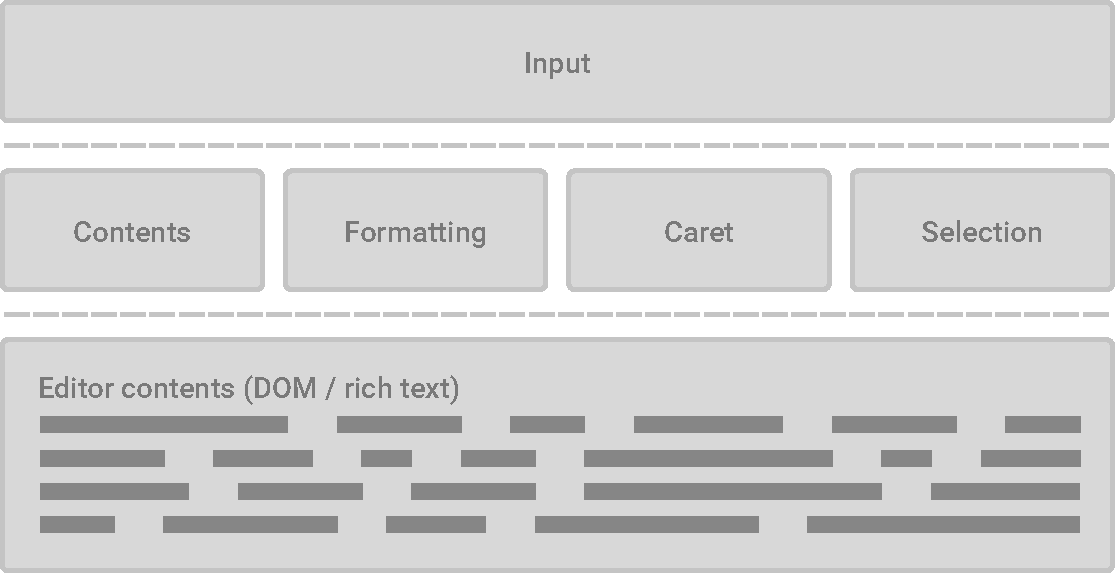
\includegraphics[width=\textwidth]{images/basic-diagram.pdf}}
\caption{Components instantiated by the Type base class}
\label{fig:type_base_components}
\end{figure}

%\begin{itemize}
%\item Contents
%\item Formatting
%\item Caret
%\item Selection
%\item Input
%\end{itemize}

\noindent The \code{Input} class will listen to keyboard input and mouse input. It is responsible for setting the caret and the selection using the \code{Caret} and \code{Selection} classes and uses them to determine which part of the text should be changed or formatted when the user enters text, uses keyboard shortcuts or uses his or her mouse or touch device. It passes formalized edit operations to the \code{Contents} class which will emit events for an \code{UndoManager} that enables undo and redo operations. The \code{Contents} class uses the \code{Writer} and \code{Formatter} instances to manipulate the visible text on the website. These classes perform the actual DOM operations on the contents of the element passed to Type on instantiation (see \refsubsec{subsec:instantiation_usage}).

%class allows adding and removing text and the \code{Formatting} class allows to apply formattings, both using DOM operations. The \code{Changes} class will use these classes to to alter the text according to the change it it should apply.

Usually, text input fields contain one caret and display one text selection at a time. For this reason the \code{Type} base class instantiates the \code{Caret} and \code{Selection} classes for shared usage within an editor's instance. Of course, this behavior can be extended, for example by instantiating multiple \code{Caret}s for real-time text collaboration.


%\noindent The \code{Contents} and \code{Formatting} classes allow to add and remove text (\code{Contents} class) and to apply text formatting (\code{Formatting} class) to the editor's contents using DOM operations. These classes solely provide functionality. The \code{Input} class will listen to keyboard input and mouse events and utilize the \code{Caret} and \code{Selection} instances to

% apply the input to the appropriate part of the text though the \code{Changes} model. These classes in turn require further classes for their implementation. Section \refsection{sec:modules} will discuss the characteristics of these classes and how they interact. %each class and its specific 


% directed acyclic graph ? 

\section{Input reading}

There are various input methods with which users can interact with native inputs. This includes using hardware devices as well as virtual (on screen) devices:

\begin{itemize} 
\item Hardware keyboard input
\item Virtual keyboard input
\item Mouse input
\item Touch input
\item Game controller input (on game consoles)
\item Remote control input (on smart TVs)
\end{itemize}

When mimicking a native input, in a best-case scenario, all these input methods should be accounted for. Fetching input includes two scenarios: The user clicks, touches or focuses the input in any way and does so at any position inside the input. If the user points (touches, clicks, etc.) in the middle of the text, the caret should move to that position. In environments without hardware keyboards, the library must ensure that a virtual keyboard shows up. Once the input is focused, text input must be fetched and written to the contents. There are various options to fetch user input, which will be discussed in the following sections.

\subsection{Events} 

One way to fetch user input is by listening to events.

\paragraph{Keyboard} Text input can be read through \texttt{KeyboardEvent}s. Keyboard events will be triggered for virtual keyboards and for hardware keyboards. When the user presses a key, the event can be stopped and the according characters can be inserted at the offset of the caret. As a downside, listeners for keyboard events cannot be bound to an element that is not a native text input, that means keyboard events must be listened to on the \texttt{document} level. This does not only have (minor) performance downsides but als requires more logic to decide whether a keyboard input should be processed and ultimately stopped or ignored and allowed to bubble to other event listeners of a website. In particular, there can be edge cases, where even though a keyboard event should write contents to the editor, the event itself is supposed to trigger other methods that are not part of the editor. Keyboard events are supported by all major browsers across all devices.

\paragraph{Mouse and touch} To support clicking or touching inside the editor's contents \texttt{MouseEvent}s and \texttt{TouchEvent}s can be used. Mouse events are supported on all major desktop browsers and all mobile browsers support touch events. Both event types support reading the coordinates indicating where the click or touch has been performed.

\paragraph{Remote controls} Although some smart TVs offer keyboards, mice, pointers similar to Nintendo's Wii remote, input via smartphone apps and many other input divides, button-based remote controls are offered with almost any smart TV and remain a edge case for interacting with a text editor. In such an environment, users commonly switch between elements by selecting focusable elements with a directional pad. Only using events would not account for this since there would be no focusable element representing the editor. Recent browsers on Samsung's and LG's smart TVs are based on WebKit\footnote{\url{http://www.samsungdforum.com/Devtools/Sdkdownload}, last checked on 07/22/2015} while Sony's TVs use Opera. Before 2012 Samsung's browser was based on Gecko. All of these browsers and browser engines support keyboard events triggered by virtual keyboards to fetch their input.

\paragraph{Clipboard} Another problem with relying entirely on events is the lack of native clipboard capabilities. Unless a native text input (including elements with enabled editing mode) is focused, shortcut keys for pasting will not trigger a paste event and the mouse's context menu will not offer an option for pasting. % \textit{Recent versions of Chrome, Opera and Android Browser\footnote{\url{http://caniuse.com/\#feat=clipboard}, last checked on 07/22/2015} allow triggering arbitrary paste events on elements in editing mode thereby read the cliboard contents. With this, shortcuts could be enabled with JavaScript and instead of the native context menu, a customly build context menu using HTML could be shown that allows the user to paste, but this only works on elements in editing mode and only in these three browsers.}

\subsection{Hidden native input fields} 

\label{subsec:hidden_native_input_fields}

As discussed in \refsection{sec:approaches_for_imitating_native_components}, the source code editors Ace and CodeMirror use a hidden (native) input field to fetch the users' keyboard input. While it appears to the users they are entering text in a syntax-highlighted representation of the source code, in reality users enter their text in a \textit{hidden} \code{textarea} element. The input will be read from the \code{textarea}, processed and displayed with syntax-highlighting using HTML. This solves many problems that occur with relying solely on events:

\begin{itemize}
\item The hidden \code{textarea} can be focused with the tab key.
\item The hidden \code{textarea} can be focused with remote controls.
\item Virtual (on screen) keyboards will show up when the \code{textarea} is focused.
\item Keyboard shortcuts for clipboard events work.
\item It can display a native context menu that allows pasting.
\end{itemize}

\subsection{Implementation}

The \code{textarea} is created when the editor gets instantiated. Since browsers scroll the \code{textarea} into view when it receives the focus, it is positioned in the visual representation of the editor, scrolling the editor into view\footnote{This does not mean the editor will be scrolled into view on instantiation, but when the user focuses ist, for example with the tab key.}. This perfectly mimics the browser's native behavior. To maintain the illusion that the user actually writes inside the visual representation of the editor the \code{textarea} is hidden.

\subsection{Focus} Whenever the user clicks inside the editors visible contents, the mimicked caret will be moved (see \refsubsec{subsec:caret}) to the according text position. To enable text input, the hidden \code{textarea} will be focused on click or touch events. The \code{textarea} is natively focusable using the tab key or a remote control on a smart TV. It will also trigger focus and blur events. This way, it is possible to display the caret when the \code{textarea} receives the focus and read its input as well as hiding the caret on blur and thereby perfectly mimic the native behavior for input events.

\subsection{Virtual (on screen) keyboard support} The \code{textarea} will be focused when the user clicks or touches inside the editor as well as with the tab key and remote controls. Focusing a text input triggers the display of native virtual keyboards.

\subsection{Pasting} 
\label{subsec:input_textarea_pasting}

When a the textarea is focused, pasting via keyboard shortcuts is natively available. To enable pasting with the context menu, CodeMirror implements a technique where the \code{textarea} will be moved to the pointer's position on a \code{mousedown} event. Following the order of \code{MouseEvent}s, this will be completed before the context menu will be triggered. This way it will be triggered on the \code{textarea} and contain a paste option. The paste event will insert the contents from the clipboard to the textarea from which the contents can be read.

\subsection{Reading input} \code{textarea} elements support \code{input} events which can be used to read the text entered by the user. The input can be processed as discussed in \refsection{sec:module_architecture} and be removed from the textarea. In practice, this means that once a single character has been entered in the \code{textarea} it will be read from the \code{textarea}, inserted into the editor's contents and the \code{textarea} will be cleared again. Input reading requires further processing before it can be passed on to trigger a change in the editor's contents. The specifics on processing the input will be discussed in section \refsection{sec:input_pipeline}.

\subsection{Editing mode} Using a \code{textarea} element allows plain-text input only. This is not a problem for regular keyboard input but rich-text contents pasted from the clipboard will be inserted as plain text and all formattings will be removed. To come around this issue, a \code{div} element in editing mode can be used instead of a \code{textarea} element.

As discussed in \refpart{part:discussion} HTML editing APIs are very problematic and a key factor of this thesis is implementing a rich-text editor without using them. However using an element in editing mode only for input reading is not affected by these issues. Whenever a single character will be entered it will be read and immediately removed from the editable element. Formatting commands will not be used at all. Problematic text input behavior, for instance different markup that will be generated by the entering a line break, will not occur since the the editable area will only be used for reading input, the text that will be inserted in the editor will be generated by the library (see \refsection{sec:input_pipeline}). The only difference between a \code{textarea} and the editable element lies in the different contents it accepts for pasting. \refsubsec{subsec:editing_disadvantages_clipboard} discusses the problem that text pasted from the clipboard cannot be processed with native APIs across all browser. In this case, the clipboard contents will be pasted to a designated field from which it can be read, isolated from the editors contents, which solves this problem (see section \refsection{sec:impl_pasting}).


%This does not cause any of the issues discussed in \refsection{sec:disadvantages_of_html_editing_apis}. Formatting and generating HTML, the related API are implemented though JavaScript and not through HTML editing APIs. The contents of the editor are not directly affected by the editing mode and its restrictions. The (known) bugs of HTML editing APIs do not affect text input or the paste event itself. The issues arise with pasting and HTML editing APIs are related to controlling process of pasting, which happens after the HTML editing API related pasting, by reading from the \code{div} element and is implemented independently of the editing API though the input pipeline (see \refsection{sec:input_pipeline}).

\section{Input Pipeline}
\label{sec:input_pipeline}

\subsection{Overview} 
\label{subsec:input_pipeline_overview}

\begin{figure}[!htb]
\centering
\makebox[\textwidth]{
\includegraphics[width=\textwidth]{images/input-pipeline.pdf}}
\caption{Input pipeline with sample filters}
\label{fig:type_base_components}
\end{figure}

Before the text read from the hidden input field will be passed on to the \code{Contents} class, it will be passed though a series of \code{Filter}s, called the ''input pipeline''. The input pipeline has 3 basic responsibilities.

\begin{itemize}
\item Stop and dispatch input that that should trigger functions of the library
\item Implement rich-text editing behavior
\item Filter and transform text
\end{itemize}

The input pipeline is part of the \code{Input} class. The pipeline itself is an array of input filters that can be added, removed and ordered with a designated API.

Input filters have a public API that specifies for which input they should be called. For instance, a filter can specify to be called when the user presses the \keystroke{ctrl}\keystroke{s} key combination. A filter can specify a handler for the input. For pressing \keystroke{ctrl}\keystroke{s}, a filter can specify to call a ''save'' function. The input is passed to the filters as an event (see \refsubsec{subsec:input_event}) that can be stopped from bubbling. This way it can be prevented that pressing \keystroke{ctrl}\keystroke{s} will also insert an ''s'' character to the editor. The order in which filters will be called is important. Some filters process the input and must cancel the event not only to prevent a character to be inserted, but also to prevent other filters from taking action.


%JavaScript does not support the concept of \code{Interfaces} and although the constructor pattern allows class-like structures, it does not support classical inheritance. Both can be implemented through supporting constructs and the \code{Utilities} class (see \refsection{sec:utilities_class}) implements a method for the latter. \textit{REWRITE CORRECT} Instead, each input filter registers and specifies for which input should be called. 
%    unless implemented with supporting constructs\footnote{Interfaces can be implemented though helper classes too}. These constructs can be costly in terms of file size and performance. For this reason, input filters do not implement a formalized interface and do not inherit a base filter class. 

The basic filters implemented for this library will be listed hereinafter, grouped by the responsibility as listed above.


%The \code{Input} class will pass any entry made in the \code{textarea}

%The \code{Input} module checks .
%Filters are classes that can be instantited and added to the 

% The order in which filters will be applied can be important

\subsection{Triggering functions}

\paragraph{Caret} Commonly, when a user presses one of the arrow keys inside a text, the caret will be moved and of course, in a browser environment, this is not different. To mimic this behavior arrow key input will be intercepted by the \code{Caret} input filter class, which will move the caret that has been instantiated by the \code{Type} base class (see \refsection{sec:module_architecture}). It will also account for modifier keys and the operating system used and move the caret accordingly.


\paragraph{Command} The \code{Command} input filter class checks for and intercepts keyboard shortcuts commonly used for text formatting. 

\begin{itemize}
\item \keystroke{ctrl}\keystroke{b} Formats the currently selected text bold.
\item \keystroke{ctrl}\keystroke{i} Formats the currently selected text italic. 
\item \keystroke{ctrl}\keystroke{u} Formats the currently selected text underlined.
\end{itemize}

To format the text, by default, the tags \code{strong}, \code{i} and \code{u} will be used. Since in some cases this might not be desired, these default keyboard shortcuts must be opted-in by setting an option on instantiation (see \refsubsec{subsec:instantiation_usage}).

The input event implements an abstraction to either check for the \keystroke{ctrl} key or the \keystroke{cmd} key depending on the operating system of the user (see \refsubsec{subsec:input_event}) so that the above-mentioned shortcuts can (only) be triggered with the \keystroke{cmd} key instead of the \keystroke{ctrl} key on the OS X systems.


\subsection{Rich-text behavior}

As discussed in \refsubsec{subsec:concept_native_imitation}, most rich-text editors support the user with a common behavior reacting to the user's input. This behavior can be abstracted in a simple way using the input pipeline. The following paragraphs describe the rules and filters implemented by default. Further rules can easily be implemented and added to the input pipeline as input filters.

\paragraph{Headlines} When a user presses \keystroke{enter} while the caret is located at the end of a headline, a new text paragraph will be created behind the headline and the caret will be placed inside it.

\paragraph{Lists} Pressing \keystroke{enter} inside a list item creates a new list item behind the current item and the caret will be placed inside it.

\subsection{Filterring and transformation}

\paragraph{Line Breaks} To display a line break in the contents of the editor a \code{br} or \code{p} tag must be inserted. When the user presses the \keystroke{enter} key it does not suffice to insert a carriage return and/or line feed. This input will be intercepted and instead a \code{br} tag will be inserted to the editor's contents. As discussed in \refsubsec{subsec:input_pipeline_overview}, it is important that this filter will be invoked after the \code{Headlines} and \code{Lists} filters, so they can apply their behavior and prevent this filter's behavior.

%\footnote{To enforce a line break other tags. like the \code{div} tag can be used, but would not be semantically appropriate in this context}

\paragraph{Remove} To delete text from the editor the \code{Remove} filter checks for \keystroke{backspace} and \keystroke{del} key inputs. Depending on whether there is a text selection or not, it either deletes the selection's contents or one character left/right of the caret.

\paragraph{Spaces} Browsers display adjacent spaces as a single space. This is an unusual behavior for text editing. The \code{Spaces} input filter checks if adjacent spaces are being entered and inserts non-breaking spaces.

\subsection{Events} As an alternative approach input filters could be implemented as input event handlers. With this, the same functionality could be achieved without an input pipeline. A designated pipeline however provides a clearer mental model for processing the input as it allows a separation of concerns. An input filter has a specific purpose and context as compared to an arbitrary input event handler. It can also be made sure that filters will be called in the right order and that any input filter will be run before triggering an input event. This way input event handlers only receive actual text input for the editors contents while keyboard shortcuts and other keypresses have been filtered out.

\subsection{Extendability} The input pipeline is intended to be extended. It serves as an entry point for other developers to process input. For this, the \code{Input} class provides an API to add, remove and reorder input filters.

%While these are the basic responsibilites 


%pipeline idea
%rules for behaviours (lists, headlines, enter, spaces...)
%Ursprünglich so gedacht: Was gehört zu einem editor X, Y und Behaviour. Für Behaviour aber das input pipeline system gefunden, welches das ganze schön abbildet/löst.
%Noch mal skimmen und sehen ob da was dabei ist, besonders "Detour": http://marijnhaverbeke.nl/blog/browser-input-reading.html

\section{Pasting}
\label{sec:impl_pasting}

As discussed in \refsubsec{subsec:hidden_native_input_fields}, all text input will be read from a designated input field. It is useful to distinguish between regular keyboard input from input pasted from the clipboard since the clipboard can contain rich text contents. Developers implementing an editor with Type should be able to determine which formattings should be allowed in the editor, i.e. pasted from the clipboard. This requires two steps.

\begin{enumerate}
\item Determine if an input has been made through typing or pasted from the clipboard.
\item Process the clipboard contents and make them accessible to developers.
\end{enumerate}

\paragraph{Paste detection} As discussed in \refsubsec{subsec:editing_disadvantages_clipboard}, modern browsers trigger paste events, which can be listened to. Not all browsers allow reading contents from a paste event, but this is not necessary. The paste paste event will insert its contents into the designated input element from which its contents can be read, after the event has completed. Some older browsers, specifically Opera versions older than 12.1 do not trigger paste events at all. For legacy support, the browser can be tested for an available clipboard API and in case it is missing, the text input can be checked for its text length. With the system discussed in \refsubsec{subsec:hidden_native_input_fields}, an input will always have the length of a single character. If the input is longer than that, this either means more than one character has been inserted or a single formatted character has been inserted\footnote{The input field will contain markup of more than one character}. These cases can only happen when contents have been pasted from the clipboard. However, if a single unformatted character has been pasted, it cannot be distinguished from a regular text input. It is to be noted that the use case this feature is designed for, is to sanitize pasted input, which is not necessary for a single plain text character input, although it must be acknowledged that there can be use cases requiring to register any paste event for other reasons.

%\footnote{This will mainly affect users of Opera version 12.1 and older.}

\paragraph{Processing} To process the pasted contents and possibly prevent inserting the contents to the editor an \code{InputEvent} will be generated and passed through the input pipeline. Any filter can be implemented to treat or ignore paste events. Users of the library can set an option on instantiation to determine how to treat pasted contents. These options include to allow plain text only, to allow any formatted text or specifying rules to allow specific formattings only. A full API description can be found at ABC. These options are implemented in the \code{Paste} filter, that will either let any contents pass through (allow any formatting) or filter out specific or all HTML tags.

%Damit rich text gepastet werden kann elememt in editing mode anstatt textarea verwedent. Kontrolle durch die Implementierung mit einem versteckten Eingabefeld. Erst mal gibt es ein reliable Paste event, was es in keinem Editor basierend auf contentEditable gibt. 2. Hat man volle Kontrolle über den Inhalt, was gepastet wird und was nicht. Und das ganze mit einer einfachen API. Pasting sollte internes event ausloesen.

% Apart from rich-text editors there are also third-party JavaScript libraries that allow embedding code editors with syntax highlighting in a website. The ''Ajax.org Cloud9 Editor (Ace)'' and ''CodeMirror'' editor are amongst the most well-known choices. Both editors keep an internal representation of the plain-text (i.e. non-highlighted) contents of the editor, parse it and display a highlighted version using HTML in a designated \texttt{div}. Both editors use a hidden \texttt{textarea} in which the user enters his or her input. The input will be read from the \texttt{textarea} and

% which is presented to the user as the input field.

\section{Caret}
\label{subsec:caret}

The \code{Caret} class provides all functionality to place and move a caret in a text. It provides methods to be moved left, right, up and down in a text as well as to be placed at at specific position in a text. The visual representation of the caret is a \code{div} element, styled to imitate a text caret. Using a CSS3 animation, it imitates the ''blinking'' common for native text carets.

It is to be noted that the elements for carets as well as for the text selection will not be written to the editor's contents. As discussed in \refsection{sec:concept_markup}, the editor's contents should not contain any markup other than for the text itself. Instead this and all other elements will be stored in a designated \code{div} element at the end of the website's \code{body} and be positioned using CSS.

 The challenge with this class is that it must be able to be moved within text and in any kind of formatting, represented by any combination of DOM nodes. To be moved across letters and text lines, the caret must take into account that:

\begin{enumerate}
\item Letters have different widths and heights
\item Different fonts have different letter dimensions
\item Different formattings like a headline, italicized text or text with a specifically set font size, result in different letter dimensions
\end{enumerate}

\code{CodeMirror} solves these problems by measuring each letter with the use of text ranges. Browsers offer a \code{Range} interface, a construct that has a start- and end-offset in a text. A range has methods to read its x- and y-coordinates on the website. These methods can be used to span a range over a single character, read its offsets and place the caret next to it using CSS and giving it the same height as the character.

To move the caret left or right, the according characters left and right of its current offset will be measured using this method. To move it up and down across text lines, the caret must check the offsets of every character, starting from the character of the current offset, until it reaches the character above or below it that is closest to its horizontal position. As discussed in section \refsection{sec:cache}, a cache to store positions cannot be applied. The complexity of this is method $O(n)$, however in practice, the number if characters this will affect is limited by readability and usability of the text editor. Mobile devices, that generally have less performance than desktop machines, have smaller screens displaying less characters per line. While this is not necessarily the case, it can be expected by good software design.

\section{Selection}

Using a designated input element for input reading comes with the cost of having to emulate the text selection. When the input field is focused, any selection on the web site, including that of the editor, will be removed. When text is selected, the input field does not necessarily have to be focused. To read inputs, it can be focused on a ''keydown'' event, which will only remove the text selection when the user enters text. This is not problematic since selections will be removed on native inputs when a user enters text too. However, if the user right-clicks in the editor, the input element will be focused to enable pasting from the context menu (see \refsubsec{subsec:input_textarea_pasting}). This will remove the text selection on any right click.

The W3C specifies an API to add multiple ranges to a selection, which should appear as multiple selections to the user. This way the element for input reading could be focused while other parts of the website, i.e. the editor's contents, could display a selection at the same time. However, while the API is available across all major browsers, it is dysfunctional and documented to not be working.

CodeMirror, ACE and Google's document editor each implement text selections by displaying \code{div} elements that mimic the look of a native selection. Type uses the same technique to show a text selection while the input element is focused. This mimicked selection replaces native selections entirely and will be created dynamically when the user clicks in the text and drags his or her mouse across the text.
%In contrast to the mentioned editors, the selection's DOM elements stored within the editor's contents to keep the content's markup clean at all times. Instead they will be written to the end of the document's body, positioned absolutely and repositioned when the browser will be resized.

The downside of this technique is that copy commands will not work anymore due to the fact that there is no actual text selection that can be copied, even though it appears to the users there is one. To treat this issue, CodeMirror adds the contents of the imitated selection to the hidden input field and selects these contents with a native selection. This allows the user to use keyboard shortcuts at any time and to copy text with the context menu. When the user types, the selected contents in the input field will be overwritten by the browser, so this does not affect input reading. Type uses the same technique.

%Fake damit copy \& past nativ funktioniert
%Obwohl eine selection mehrere Ranges haben kann, wird das von keinem Browser unterstützt http://stackoverflow.com/questions/4777860/highlight-select-multiple-divs-with-ranges-w-contenteditable/4780571\#4780571
%Habe versucht mit die Darstellung über getClientRects zu emulierten, aber das ist buggy siehe https://github.com/edg2s/rangefix/blob/master/rangefix.js


%\paragraph{Selection Overlay}
%overlay


\section{Contents}
\label{sec:contents_impl}

The \code{Contents} class provides an API to add, remove and format text. This functionality is implemented through the \code{Writer} and \code{Formatter} classes. Its central responsibility is to proxy commands to these classes and to create ''actions'' to pass them on to the \code{UndoManager}. An action describes the formatting, change or deletion of contents in a formalized way that can be undone by the \code{UndoManager} (see \refsection{sec:undo_manager}).

%The \code{Contents} class provides an API to add, remove and format text. This functionality is implemented through the \code{Writer} and \code{Formatter} classes. Its central responsibility is to proxy commands to these classes and to trigger \code{ChangeEvent}s (see \refsubsec{subsec:change_event}) that contain a formalized description of the edit operation. \code{ChangeEvent}s will be observed by the \code{UndoManager} (see \refsection{sec:undo_manager}) to implement undo / redo functionality.

%This architecture has been chosen not only to achieve a decoupled software architecture with a clear separation of concerns, but to allow extensions to observe content changes. % For instance, the Etherpad extension uses this to populate changes to other clients (see \refsubsec{subsec:etherpad_type_client_implementation}).

%Apart from a separation of concerns, this architecture allows for extensions and possible future internal use cases to perform edit operations either directly, by using the \code{Writer} and \code{Formatter} independently of the \code{Contents} class

%Its central responsibility is to keep track of these changes and provide an API for \code{ChangeListener}.

%All components should be usable by extensions, that's one of the big reasons why it should be ausgelagert, apart from software architecture


\subsection{Writer}

The \code{Writer} class implements functionality to add and remove contents to and from the editor. Along with the \code{Formatter} class, this is the lowest layer of the editor that will perform DOM operations to modify the contents in the browser.


\subsection{Formatter}

The \code{Formatter} is one of the key classes of the Type library. As discussed in \refsubsec{subsec:noapi_dis_formatting} it must generate \textit{well-formatted} markup while being able to work on any \textit{ill-formatted} markup it will be given. There is a virtually infinite number of edge-cases for markup that formatting commands can be applied to. Assume we have the following string.

%\begin{quotation}
%Lorem \tikzmarkin{a}ipsum \textit{dolor \underline{sit\tikzmarkend{a} amet}}
%\end{quotation}

%And we want to format the highlighted part (yellow) with an arbitrary tag. Its 

 %It does not only need to deal with different markup, these edge cases also include formatting with different tags and on different parts of the same markup. %the number of edge cases is virtually unlimited

\begin{lstlisting}[language=html, caption=Markup with highlighted target for formatting, label=lst:formatter_code_example]
<p>Lorem §\tikzmarkin{glw}§ipsum <em>dolor<u> sit§\tikzmarkend{glw}§ amet</u></em> consec</p>
\end{lstlisting}

\reflisting{lst:formatter_code_example} represents markup for the formatted string ''Lorem ipsum \textit{dolor \underline{sit amet}}''. The highlighted part (yellow) represents the part of the text that should be formatted using a formatting command.

\begin{figure}[!htb]
\centering
\makebox[\textwidth]{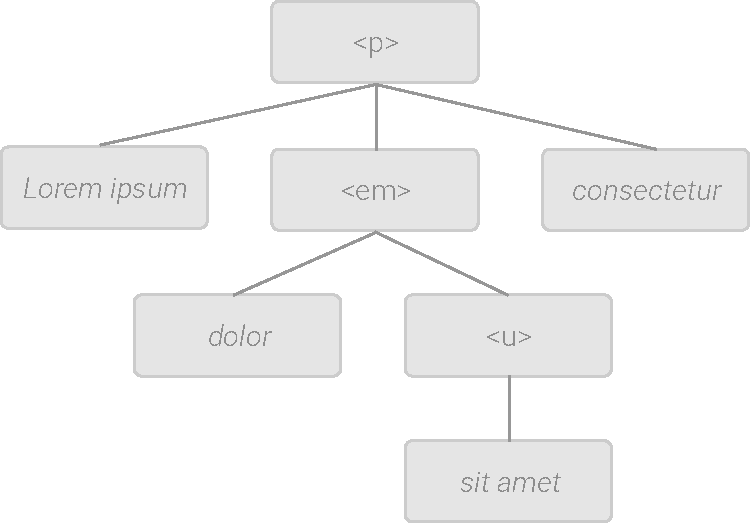
\includegraphics[width=0.5\textwidth]{images/dom-tree.pdf}}
\caption{DOM representation of figure \ref{lst:formatter_code_example}}
\label{fig:formatting_dom_tree}
\end{figure}

\reffigure{fig:formatting_dom_tree} shows the DOM representation of the markup of \reflisting{lst:formatter_code_example}. We can split up the text node ''Lorem ipsum'' into two text nodes ''Lorem'' and '' ipsum'' to create a distinct node in which the formatting (yellow highlight) starts and do the same with the ending text node ''sit amet''. This gives us a distinct nodes for the start and the end of the selection. When we traverse each node from the start to the end, every traversed node falls on either of the following cases:

\begin{enumerate}
\item It is the start node
\item It is the end node
\item It is a node between start and end node (but is not and does not contain the start or end node)
\item It contains end node
\end{enumerate}

\noindent To generate \textit{well-formatted} markup as discussed in \refsubsec{subsec:noapi_dis_formatting}, the following 2 rules must be followed:

\begin{enumerate}
\item The markup must conform the validation rules of HTML as specified by the W3C.
\item The markup must use as little DOM nodes as possible.
\end{enumerate}

\begin{algorithm}
\caption{Recursive algorithm to apply text formatting}
\label{alg:text_formatting}
\begin{algorithmic}[1]
  \Procedure{Format}{$s,e$}\Comment{s and e are the distinct start and end nodes}
    \State $c \gets s$
    \State Let $a$ is an empty array
     \While{$c\not=null$ and $c\not=e$ and $c$ does not contain $e$}
      \State $a$.push($c$)
      \State $c \gets c$.nextSibling
     \EndWhile
     \If{$c=e$}
      \State $a$.push($c$)
     \EndIf
     \If{$c$ contains $e$}
      \State \Call{Format}{$c$.firstChild, $e$}
     \EndIf
     \If{$c=null$}
      \State $n \gets $ next node in document flow
      \State \Call{Format}{$n,e$}
     \EndIf
     \State Wrap all nodes from $a$ with DOM node to apply formatting
     \State Connect siblings to wrapping node if they have the same tag
  \EndProcedure
\end{algorithmic}
\end{algorithm}

\refalg{alg:text_formatting} demonstrates a recursive algorithm, that will start iterating from the given start node over all its subsequent siblings until there are no siblings anymore \textit{or} it found the end node \textit{or} it found a node containing the end node.

\begin{itemize}

\item If the end node was found, the algorithm will wrap all all nodes it found with a node that applies the desired formatting.

\item If there are no more siblings, it means it has reached the last sibling inside the node containing the start node. By the validation rules of the W3C, nodes are not allowed to intersect. The algorithm will wrap all nodes it found so far with a node that applies the desired formatting and recursively applies itself with the start node being the next node in the document flow and the end node remaining the same end node.

\item If an element has been found that contains the end node, the algorithm will wrap all nodes it found so far with a node that applies the desired formatting (to avoid intersecting nodes). It will then apply the formatting algorithm recursively to the first child of the containing node. If this node in return is another container to the end node, the recursion will repeat until a sibling of the end node or the end node itself has been found.

\end{itemize}

Each rule performs the minimally necessary steps to format contents while conforming the HTML validation rules of not intersecting DOM nodes. By adding only the minimum of nodes, this will ensure simple (and valid) markup.

To format the nodes that have been collected by the algorithm, they will be wrapped by a DOM node that applies the desired formatting. The wrapping function will also remove any nodes between the start and end node that have the same tag as the node used for the formatting to clean up the markup. If the start or the end node has been contained by a node of the same tag as the node the text should be formatted with, the containing nodes will be used as start or end node. As a last step to improve the markup, the nodes left and right of the formatting node will be unified with the formatting node, if they have the same tag. These steps will simplify potentially \textit{ill-formatted} markup that the formatting command affects. All DOM manipulations will be performed at the end of the algorithm, when all nodes have been read to improve performance.

%    \State Split start end end text nodes to generate distinct start end end nodes
%\andnext does not contain end node

%when we create distinct start and end nodes and traverse node from the start to the end node
%we can break it down to these / is always one of these patterns: 

%- is the start node
%- is the endnode
%- is between start and end node
%- contains end node

%this way we can write a recursive algorithm

%to create clean code at the end we check if the nodes before and after the new formatting have the same formatting and connect those (whitespace nodes in between will be ignored)

%to improve performance we collect all these nodes an perform the minimum of dom operations necessary

\section{Undo Manager}
\label{sec:undo_manager}

The \code{UndoManager} implements the undo and redo functionality of the editor. It can receive ''actions'', which are instances of classes inheriting from the \code{Type} action base class. Each instance has the methods \code{execute} and \code{undo} to apply and revoke its particular functionality. There are 3 types of actions.

\subsection{Insert}

The \code{Insert} action will insert text on execution and delete the text when its \code{undo} method will be called. It utilizes the \code{Writer} class for these operations. It must be instantiated with the according text so it can be executed and undone at any time.

\subsection{Remove}

The \code{Remove} action will remove text on execution and store it to insert it again when it is being undone. Just like the \code{Insert} action it uses the \code{Writer} class for this.

\subsection{Format}

The \code{Format} action applies formattings using the \code{Formatter} class. It will store references to the nodes the \code{Formatter} created to remove them when the action will be undone.

\subsection{Stack}

The \code{UndoManager} stores each action to an array (the undo stack) so that each action can be undone and redone in order. In some cases, consecutive actions, like multiple insertions, should be undone in a single undo command invoked by the user. For this, each action must implement the methods \code{mergable} and \code{merge}. When an action get added to the \code{UndoManger} the \code{mergable} of the highest element in the undo stack will return if it accepts the new action to be merged with it. The \code{Insert} action will accept other instances of the \code{Insert} action class so that consecutive character input can be undone in chunks and not only in characters. Each action will implement merging with other instances in its \code{merge} method to which a new action will be passed if \code{mergable} returned \code{true}. Otherwise the new action will be added to the undo stack. The \code{UndoManager} will only merge actions that have been passed within a time frame of 500 milliseconds, to generate a distinct undo history.

%When an action get added to the \code{UndoManger} it passes the action to the \code{mergable} method of the highest element in the undo stack, which then returns if it accepts the action should be merged with itself. The \code{Insert} action will return true if will be passed another instance of the \code{Insert} action and false for all other actions. The \code{UndoManager} will pass the new action to the \code{merge} method 

\subsection{Action sources}

The Etherpad extension (see \refsection{sec:etherpad}) allows multiple users to modify the same text. The undo methods must only undo changes from the user that initiated the action. Furthermore, undoing and redoing an action must account for changes that affect the action, for instance, when the offset at which a text has been inserted has shifted, because another user has inserted text before that offset. To manage this, each action contains a source identifier that will be generated by the \code{UndoManager}. With this identifier the \code{UndoManager} can choose to undo actions of a particular user and account for changes of actions from other users.


%The \code{UndoManager} class will observe \code{ChangeEvent}s (see \refsubsec{subsec:change_event}) and keep a history of the performed changes. Every change must include an identifier of the source of the change. The \code{Contents} class will declare the \code{Input} class as the source for the change. This is to enable extensions to work with the \code{UndoManager}. The Etherpad extension (see \refsection{sec:etherpad}) will change the editor's contents too. If, at a given time, the local user added some text and after that another connected client would add some text a few characters before the local user's change, the \code{UndoManager} must account for both changes to undo the local user's change.

%\subsection{Change Listener}

%In its core the changes observed by the \code{UndoManager} will be kept track of by the \code{ChangeListener}. It will accumulate every change in a data structure and take a ''snapshot'' every 500 milliseconds and store it in a history. The \code{UndoManager} uses this history to implement and offer undo and redo commands.

%This functionality has been abstracted to be reused by other extensions. The Etherpad extension uses this class to accumulate and publish local changes every 500 milliseconds to its connected clients independently of the \code{UndoManager}.

%\subsection{Undo / Redo}

%The \code{Change} event can contain operations to

%\begin{itemize}
%\item Insert or remove text
%\item Format text
%\end{itemize}

%Inserting and removing can be undone easily by performing and insertion to undo a remove operation and vice versa. Formatting text is more difficult since Type allows formatting with arbitrary markup. This can be solved by keeping track of the offsets and characters affected by the formatting command and removing the HTML tags at the corresponding positions.



%The \code{UndoManager} will keep track of all changes and take a ''snapshot'' every 500 milliseconds and store it in its history. It offers an API to to undo and redo changes based on this history. 


%Has been abstracted to decouple functionality from undo/redo functionality to be reused by other developers and with the etherpad extension in mind.

\section{Events}
\label{sec:events}
\subsection{Overview}

It is possible to trigger custom (native) events using the \code{CustomEvent} interface on modern browsers\cite{mozev}. Internet Explorer 9 and below allow this through similar interfaces. These interfaces could be used for triggering events for components of Type. However, this would trigger events that that are only relevant within the library in the global namespace. To avoid this, Type implements its own event system that populates events only within the library. Events from within the editor that can be useful to the website or web application should still be triggered as native events in the browser's global namespace. %During the development of the library no such use case has occurred.

%\footnote{\url{https://developer.mozilla.org/en/docs/Web/API/CustomEvent\#Browser_compatibility}}

%\textit{todo explain browser support}

%Dazu entscheiden dass es ein Type-Internes Eventsystem gibt, dessen Events nur in Type existieren. Damit polluten die nicht den globalen (name)space mit events. Nur bestimmte events werden global (nativ) getriggert, und das sind genau die events, die nach aussenhin von Belang sind und abgegriffen werden koennen sollen (=API design)

\subsection{Event Api}

The \code{EventApi} class provides an API to add and remove event listeners as well as to trigger events. It provides instance and static methods.

\begin{lstlisting}[language=JavaScript, caption={EventApi methods}, label=lst:eventapi_methods]
// Static methods
EventApi.on(eventName, eventHandler);
EventApi.off(eventName, eventHandler);
EventApi.trigger(eventName, eventObject);

// Instance methods
EventApi.prototype.on(eventName, eventHandler);
EventApi.prototype.off(eventName, eventHandler);
EventApi.prototype.trigger(eventName, eventObject);
\end{lstlisting}

%\begin{itemize}
%\item \code{trigger} 
%\item \code{on}
%\item \code{off} 
%\end{itemize}

Using the \code{OOP} class (see \refsection{sec:oop_class}), these methods will be inherited by the \code{Type} class. This way, using the \code{trigger} method, events can be triggered within the scope of a \code{Type} instance and be observed using the  the \code{on} method. Event handlers can be removed using \code{off} method.

The static methods will also be inherited by the \code{Type} class. This is necessary to trigger events that are \textit{Type} specific but not \textit{instance} specific. Most importantly a ''ready'' event will be triggered on every instantiation of the \code{Type} class. This way plugins and other third-party scripts can run initialization routines.

%The first parameter for any of these methods is always the event name that should be listened to, stopped to be listened to or triggered. The second parameter of the \code{trigger} method is an event object that can be an instance of any of the classes discussed in sections \refsubsec{subsec:type_event} through \refsubsec{subsec:paste_event}. The second parameter of the \code{on} and \code{off} methods can be a \code{Function} that will receive the object, that has been passed to the trigger method, as first parameter.

Plugins and third-party libraries can trigger arbitrary events and pass along arbitrary data. As a paradigm and in terms of a \textit{good programming style}, event objects should be passed. Event objects are inherited from the \code{TypeEvent} or conform its API.

\subsection{TypeEvent}
\label{subsec:type_event}

\begin{lstlisting}[language=JavaScript, caption={TypeEvent API}, label=lst:eventapi_methods]
// Gets or sets data
TypeEvent.data([options]);

// Stops the event from bubbling
TypeEvent.cancel();
\end{lstlisting}

The \code{TypeEvent} is a generic, general-purpose event. It can store arbitrary data and offers an API to be stopped from bubbling. A full API description can be found in Listing XY.

\subsection{InputEvent}
\label{subsec:input_event}

The Input \code{InputEvent} will be triggered by the \code{Input} class after a keyboard input has passed the input pipeline. It inherits all methods from the \code{TypeEvent} to conform the event system and contains information on the key and the modifier keys pressed. The key is represented with its key code and a key name. They key name will be mapped from the key code and is implemented with a list of readable names including ''backspace'', ''enter'', ''space'' and others. The list not complete but can be extended during further development. The modifier keys include ''shift'', ''alt'', ''ctrl'' and ''meta''. ''meta'' is the browser's name for the \keystroke{cmd} key on OS X systems. OS X uses the \keystroke{cmd} key as modifier the same way Windows and Linux use the \keystroke{ctrl} key. To support developing an editor for both platforms the ''cmd'' modifier will be set when a user holds the \keystroke{cmd} key on OS X \textit{or} the \keystroke{ctrl} key on other platforms.

\subsection{PasteEvent}
\label{subsec:paste_event}

The \code{PasteEvent} will be triggered when the user pastes contents from the clipboard \textit{before} it will be inserted to the editor's contents. It contains the clipboard's contents and can be cancelled so that other developers are free to manipulate and stop a paste event.

%\subsection{ChangeEvent}
%\label{subsec:change_event}

%As discussed in section \refsection{sec:contents_impl}, a \code{ChangeEvent} will be triggered when changes have been made to the editor's contents. It contains an array of formalized data structures describing the changes that have been made. There are two types of data structures, one for text insertion and removal and one for text formatting.
%
%\begin{lstlisting}[language=JavaScript, caption={Data structure for insert and remove operations}, label=lst:add_remove_structure]
%{
%    "offset": 10,
%    "operation": "insert",
%    "contents": "Lorem ipsum",
%}
%{
%    "offset": 10,
%    "operation": "remove",
%    "contents": "Lorem ipsum",
%}
%\end{lstlisting}

%Lines 1--5 in \reflisting{lst:add_remove_structure} show the data structure for an insert operation.

%\begin{lstlisting}[language=JavaScript, caption={Change data structure}, label=lst:format_structure]
%{
%    "offset": 10,
%    "characters": 5,
%    "operation": "format",
%    "parameters": "<strong />",
%}
%{
%    "offset": 10,
%    "characters": 5,
%    "operation": "removeformat",
%    "parameters": "<strong class='important' />",
%}
%\end{lstlisting}

%These data structures contain the information to undo user input and to redo the same input again.


\section{Utility classes}

\subsection{OOP}
\label{sec:oop_class}

The \code{OOP} class extends the constructor pattern with basic classical inheritance. It provides the method \code{inherits} that will duplicate and copy the \code{prototype} from one \code{Function} object to another. It also copies attributes and methods defined on the \code{Function} object itself to implement inheritance of static definitions. It adds the attribute \code{\_super} to the inheriting \code{Function} object referencing its parent class to enable child classes to access their respective superclasses.

%The \code{OOP} class implements a simple approach to extend the contructor pattern with basic classical inheritance. It does so by providing an \code{inherits} method, that copies all methods and attributes from one prototype of a class to another. In this simplified apporach, parent methods cannot be called from child classes with a unique keyword (like ''super'') as it is the case with Java or other languages using classical inheritance.

%Any static methods and attributes of a class will also be inherited by coping any method and variable defined on the \code{Function} object passed.


\subsection{Range}

The \code{Range} class is an abstraction for the native \code{Range} interface. The native implementation is prone to bugs on many browsers. Instead of fixing the API by shimming its methods, the \code{Range} class implements all methods related to ranges while trying to interact as little as possible with the native API. On top of the methods of the native \code{Range} interface, this class implements additional methods required for Type.

%As discussed in \refsection{sec:interaction_with_browser_apis}, 

%CodeMirror uses (native) \code{Range}s for text

%Ranges are specifically used to 

%Ranges are mainly used by the implementations of the caret and the selection.




\subsection{Dom Walker}

Working with text implies having to traverse the DOM, i.e. the nodes inside the text often. The \code{DomWalker} utility class solves this problem. The DOM API offers methods to access a node's siblings, children and parents, but it must always account for cases when any of these are \code{null} (there is no parent, sibling or child) or when they overflow the bounds of the editor's contents. But more importantly, for text editing, it is usually necessary to access the next (or previous) node in the document's content flow which can either be the parent, sibling, child or a node that can only be accessed by traversing multiple nodes. Also, it is often the case that it is not only necessary to fetch the next node, but to apply a filter to only fetch a specific node, for instance a text node or only a text node that has contents visible to the user\footnote{Any text node consisting of whitespace only will not be displayed by any major browser}. Browsers offer a native API for this, called \code{TreeWalker}, but it is said to be slow\footnote{\url{http://jsperf.com/qsa-vs-node-iterator}}, only partially supported by Internet Explorer 9\cite{moznode} and has been criticized for its verbose API\footnote{By John Resig, author of jQuery, \url{http://ejohn.org/blog/unimpressed-by-nodeiterator/}, last checked 08/19/2015}.

% \footnote{\url{https://developer.mozilla.org/en-US/docs/Web/API/NodeIterator\#Browser_compatibility}}

The \code{DomWalker} can be instantiated by providing a starting node and the type of nodes it should traverse. The latter argument can either be a string identifying a pre-made filter of the Type library or a custom filter function. Pre-made filters include:

\begin{itemize}
\item ''text'' - A text node with visible contents
\item ''textNode'' - Any text node, visible or invisible
\item ''visible'' - Any visible DOM node
\end{itemize}

A \code{DomWalker} instance offers the high-level methods \code{next}, \code{previous}, \code{first} and \code{last} (amongst others) for traversal. A full API description can be found in XYZ. All methods can be called statically without having to instantiate a \code{DomWalker}.

%\paragraph{API}

%The \code{DomWalker} class offers high-level methods for traversal, designed to quickly apply the most common filters. I can be instantiated with multiple shorthand parameters.

%\begin{algorithm}
%\caption{Simplified text formatting pseudocode}
%\label{alg:format_pseudocode}
%\begin{algorithmic}[1]
%\State new DomWalker(startNode, node);
%\State new DomWalker(startNode, 'filtername');
%\State new DomWalker(startNode, filterFunction()\{\});
%\State new DomWalker(startNode,\{optionsObject\});
%\end{algorithmic}
%\end{algorithm}

%\noindent The API is not only designed for the development of this library but most importantly to be a utility too for developers extending the library or implementing editors.

%The API is designed for an easy and high-level usage to simplify the workflow for developing the library, but most importantly to offer a high-level and easy-to-use concept to other developers.

%dom walker. Used SO OFTEN in the project. Goal is to have a really simple api new DomWalker('text') by having lots of pre-defined magick in it.

\subsection{Text Walker}

The \code{TextWalker} class acts as a container for all functions related to measuring text offsets. It provides utility methods to determine the character offset from one text node to another or, vice versa, which text node can be found at a text offset, starting from another given node. Both methods are required by various classes and are thus, centralized. 

\subsection{Dom Utilities}

The \code{DomUtilities} class encapsulates common methods for all DOM operations other than traversal. It has no inherent purpose but many other classes perform the same DOM operations, which hence reside in a common library to avoid code duplication.

\subsection{Utilities}
\label{sec:utilities_class}
The \code{Utilities} class is a general-purpose class that contains methods to extend JavaScript's features. It contains methods to work with data structures and to detect object types.

\subsection{Environment}

The \code{Environment} class checks and provides informations on the current browser environment and its features. This class is especially important to mimic native behavior for user interaction. For instance, as discussed before, either the control key or the command key should be used to implement keyboard shortcuts depending on the operating system. To check for specific feature support, it is favorable to use duck typing within each class.

%\section{Plugin Api}
%plugin api
\subsection{Settings}

The settings class stores settings required for Type's modules, for instance the \code{id} of the DOM-container which all helper DOM-nodes from other classes will be appended to.

\subsection{Development}

The \code{Development} class is intended to contain utility methods to support the development of the library. As for the development of this thesis, it was sufficient to implement logging methods.


\section{Cache}
\label{sec:cache}

For traversing the text, for example when the caret moves, the text will need to be measured. All measurements can be stored to a cache to only perform the same measurement operations once. When the user edits the contents of the editor, these texts will change and the cache must be updated. A cache must also account for external changes. The DOM3 Events specification\cite{UIEV} offers \texttt{MutationObserver}s to check for DOM changes. This feature is not supported by Internet Explorer version 10 or less\footnote{\url{http://caniuse.com/\#search=mutation}, last checked on 07/21/2015}. Internet Explorer 9 and 10 offer an implementation for \texttt{MutationEvent}s\footnote{\url{http://help.dottoro.com/ljfvvdnm.php\#additionalEvents }, last checked on 07/21/2015}. The W3C states that ''The MutationEvent interface [...] has not yet been completely and interoperably implemented across user agents. In addition, there have been critiques that the interface, as designed, introduces a performance and implementation challenge.''\cite[Legacy MutationEvent events]{UIEV}. For this reason, the editor does not use any caching. Implementing an editor that is stateless in regards of its contents can also improve stability.

% \footnote{\url{http://www.w3.org/TR/DOM-Level-3-Events/}, last checked on 07/21/2015}
%\footnote{\url{http://www.w3.org/TR/DOM-Level-3-Events/\#legacy-mutationevent-events}, last checked on 07/21/2015}

%Apart from that, the benefits of a cache may not significantly increase the library's performance. The actions that can be supported by a cache, most importantly moving the caret in the text, are not very complex and do not noticeably affect the CPU.


% It should be agnostic to the editor's contents at all times to give other developers the freedom to change the contents in any way needed without breaking the editor.
% On the other hand, the library should be a ''good citizen'' on a website, which means it should be as unobtrusive and leave the developers as much freedom as possible. 

\section{Real-time collaboration with Etherpad} 
\label{sec:etherpad}

\subsection{Overview}

To achieve real-time collaboration with multiple Type editors, Etherpad\footnote{Etherpad has been completely rewritten under the name Etherpad Lite. However, its official website no longer links to its former source code. For simplicity, the name Etherpad will be used, referring to its rewrite as Etherpad Lite} can be used. Etherpad is a web-based collaborative real-time text editor with rich-text capabilities. It provides a server, written in JavaScript using Node.js as well as a web-based rich-text editor. Both components are distributed in one package and are meant to be used together.

To achieve real-time rich-text collaboration, multiple web-based clients communicate with a server via WebSockets using socket.io. Each client owns a local version of the document that it needs to sync with the server. The server uses an operational transformation algorithm to merge each change to the document accounting for all changes and then urges each client to update their local contents according to the final document.

\subsection{Changesets}

For this, Etherpad uses the concept of so-called ''changesets''. Each client sends its local changes, debounced to an interval of 500 milliseconds, as a serialized string---the changeset---to the server. The changeset includes all text insertions, removals and formattings of the last time frame. Along with the changeset, it sends a document revision number that the changeset is based on to the server. The document revision number increases with every changeset that has been accepted and applied to the document on the server side. The document on the server side is saved as a stack of changesets, which ultimately form the current document. For performance reasons, snapshots can be taken that save the document as formatted text. 

Based on the revision number that the client provides with the changeset, the server can apply it to the version of the document the client was working on. The server will apply the resulting changes to all newer revisions of the document (if present) and send a changeset and the latest revision number back to the client. The changeset sent to the client includes all operations it needs to perform to update its local version to the newest version on the server.

%The changeset it sends back includes the differences from the the client's current revision of the document (with its own changes already applied) to the the latest revision on the server that includes the result of all changes the server had to perfom along each revision as just described.

As a last step, the client must apply the changeset it got from the server to its local document to display the most recent version to the user and update its local revision number to what it got from the server.

\subsection{Merging}

In a collaborative environment, it can happen that two (or more) clients send different changesets to the server that are based on the same document revision. It is the responsibility of the server to merge both changes so that it preserves either intend. As explained in the ''Etherpad and EasySync Technical Manual''[citation needed], to solve this, for a document $X$ with the conflicting changesets $A$ and $B$, the server computes the new changesets $A'$ and $B'$ such that
$$XAB' = XBA' = Xm(A,B)$$
where $Xm(A,B)$ is the merge of $A$ and $B$ applied to the document $X$. The changesets $A'$ and $B'$ will be sent to the respective clients, which will apply it to their local documents to sync with the document on the server. To compute a changeset $A'$

\begin{itemize}
\item Insertions in $B$ become retained characters in $A'$
\item Insertions in $A$ stay insertions in $A'$
\item Retain whatever characters are retained in \emph{both} $A$ and $B$
\end{itemize}

For $B'$ this applies vice versa. %This implies that anything affected by the changesets and is not inserted or retained will be removed. \textit{// CHECK ON THIS AGAIN!}

\subsection{Etherpad Client implementation}

Clients interact with the server via WebSockets using socket.io. To sync their own changes with other clients, a client does 4 things.

\begin{itemize}
\item Request a the full document from the server
\item Send a changeset to the server
\item Receive acknowledgement from the server for a submitted changeset
\item Receive a changeset from the server submitted by another client
\end{itemize}

\noindent When Etherpad's client connects to the server it receives an initial snapshot of the entire document as a string. To submit changes, the client uses a three-step architecture. The client stores any local changes that have not been sent to the server yet in a changeset $Y$. Any changeset sent to the server must be acknowledged by the server as it has applied  the changeset to its document. Any changeset that has been sent and not been acknowledged yet will be stored in a as the changeset $X$. The document as it is acknowledged by the server is stored in a changeset $A$. The document visible to the users can be expressed by the representation of $Y \cdot X \cdot A$, i.e. applying each changeset to the next.

Whenever a user applies a local change, the changeset $Y$ will be updated. Every 500 milliseconds, but not before a changeset submitted to the server as been acknowledged, the changeset $Y$ will be sent to the server and $Y$ will be assigned to $X$. $Y$ will be set to a changeset that contains no changes. When the client hears the acknowledgement for $X$ from the server, $X$ will be applied the changeset $A$ and $X$ will be set to contain no changes.

This architecture supports receiving changesets from other clients as they must be applied to a client's local changes (committed and uncommitted) as well as the document version as acknowledged by the server. When a client receives another client's changeset $B$ it will perform 4 steps.

\begin{enumerate}
\item Compute a new changeset by merging $Y (X \cdot B)$ and apply it to the document visible to the user.
\item Apply $B$ to $A$.
\item Compute a new changeset by merging $B$ and $X$ and assign it to $X$
\item Compute a new changeset by merging $(X \cdot B) \cdot Y$ and assign it to $Y$
\end{enumerate}

The operations needed to merge the changesets on the client, are the same operations for merging changesets on the server.

\subsection{Type Client implementation}
\label{subsec:etherpad_type_client_implementation}

Etherpad's technology can be used to enable real-time collaboration for Type. While Etherpad offers a web-based client, its implementation has three flaws:

\begin{enumerate}
\item It cannot be integrated easily in other web applications.
\item It does not generate semantic markup. It is cluttered with control sequences.
\item It's hard to extend.
\end{enumerate}

Etherpad does not provide a documentation on its client--server protocol, but it can be reverse engineered. It is possible for third-party libraries to communicate with an Etherpad server alongside Etherpad's ''native'' clients, as long as a third-party library (like Type) conforms the protocol.

Etherpad's collaboration functionality comes with a cost in file size for Type and may only be used in specific use cases. This is why this feature is implemented as an optional extensions (compare \refsection{sec:extensions}) in a separate file. To enable collaboration the designated JavaScript file needs to be added to the website.

\begin{lstlisting}[language=html, caption=Enabling real-time collaboration to Type, label=lst:add_etherpad_html]
<script src="type.js"></script>
<script src="type.etherpad.js"></script>
\end{lstlisting}

\code{type.etherpad.js} adds the classes it requires to the \code{Type} namespace and adds a static constructor to the Type library:

\begin{lstlisting}[language=JavaScript, caption=Static constructor to generate a collaborative Type instance, label=lst:etherpad_constructor]
var element = document.getElementById("myElement");
var editor = Type.fromEtherpad(element, "http://example.com/editor/myEditorId");
\end{lstlisting}

The constructor used in line 2 of \reflisting{lst:etherpad_constructor} will connect to an Etherpad server and load the contents of a document and append them to the element given as first argument.

\textit{Todo Will use the change listener to watch changes. Has an own class to serialize changesets. One class for pushing changes to the server. Uses caret class to display other collaborators. And has a class to apply incoming changes.}

This architecture provides an unobtrusive way to integrate real-time collaboration in the Type library. It does not depend on a specific implementation of an editor. Developers are free to implement any editor specific to their needs with integrated real-time collaboration.

% Collaboration with etherpad ist wirklich einfach zu machen mit meinem coolen editor. Mein Editor ist ganz ganz toll dass das so einfach geht, ja!



\section{Extending}
\label{sec:extensions}

\subsection{Overview}

Type's modular structure is designed for extension. Type's \code{prototype} has been exposed as \code{Type.fn} and all its classes in the \code{Type} namespace. This provides other developers with all of Type's functionality in a structured and accessible manner. Type is designed to lower the barrier for and encourage developers to extend Type by giving freedom and possibilities in how to implement an extension and trying to avoid compulsorily use of interfaces or configurations.

jQuery demonstrates a similarly liberal approach for writing extensions and experience shows that name conflicts are minimal and ''good'' extensions are naturally favored over ''bad'' extensions by the community of web developers.

\subsection{API extension}

\begin{lstlisting}[language=JavaScript, caption=Example Type instance API extension, label=lst:api_extension_example]
Type.fn.myMethod = function () {};
\end{lstlisting}

As discussed in \refsubsec{subsec_fn_exposal}, to add a method to Type's public API, its base class' prototype can be extended with a function using the \code{Type.fn} shorthand attribute. Static constructors can be added by extending the \code{Type} \code{Function} object.

\begin{lstlisting}[language=JavaScript, caption=Example custom static constructor, label=lst:example_static_constructor_extension]
Type.myConstructor = function () {
  return new Type();
};
\end{lstlisting}

\subsection{Namespace extension}

As discussed in \refsubsec{subsec:namespace_and_refs}, to implement extensions for Type, the \code{Type} namespace can be used to add custom classes or sub-namespaces.

\begin{lstlisting}[language=JavaScript, caption=Example Type namespace extension and usage of a built-in class., label=lst:namespace_extension_example]
Type.MyClass = function () {
  var caret = new Type.Caret();
};
\end{lstlisting}

%Type.MyPluginNamespace = {};
%Type.MyPluginNamespace.Foo = function() {};
%Type.MyPluginNamespace.Bar = function() {};

\noindent All other classes that Type uses are exposed in this namespace and can be used by extensions.% This can be used to provide other developers with functionality and / or to support API extensions.

\subsection{Plugin API}

A plugin may need to be initialized when an editor will be instantiated. To support this, Type will trigger an event on instantiation and pass the Type instance to the event handler

\begin{lstlisting}[language=JavaScript, caption=Example event handler for a Type instantiation, label=lst:instantiation_even_handler_example]
Type.on('ready', function(typeInstance) {});
\end{lstlisting}

\noindent To store and read data specific to an instance, Type offers the \code{data} method, that will return an \code{Object} for arbitrary access.

\begin{lstlisting}[language=JavaScript, caption=Example calls to format text, label=lst:format-examples]
Type.fn.myMethod = function () {
  this.data("myPlugin").foo = 'bar';
  var bar = this.data("myPlugin").foo;
};
\end{lstlisting}

\noindent To give each plugin an own namespace, an arbitrary identifier must be passed as a \code{String} to the \code{data} method, which will provide a unique \code{Object} for different string identifiers. This can possibly cause name conflicts if two plugins choose to use the same string. Developers are advised to always use their own extension name as identifier. Experience with jQuery's plugin system as well as jQuery's \code{data} method shows that while this cannot prevent name conflicts, it is rarely a problem.

% Erstellung von Erweiterungen und Plugins soll so einfach und frei wie möglich sein. Es ist die Verantwortung der Programmierer diese Freiheit so zu nutzen, dass sie trotzdem sauber arbeiten. jQuery zeigt, dass Freiheit funktioneren kann und nicht zu schlechtem nutzen führt. Schlechte Plugins sterben durch die Dynamik des ''Marktes'' aus. Die Vorteile ueberwiegen: Beim CKEditor ist es aufwändig (viel Code um sich in den Editor zu integrieren) und schwierig (Lernkurve) Erweiterungen zu schreiben. Der CKEditor ist aber auch ein Produkt und kein Framework. Ein Framework sollte Möglichkeiten geben und einfach (und painless) sein. jQuery hat für sich Konventionen erzeugt und Möglichkeiten gegen, die Programmierer effektiv arbeiten lassen können. Und jQuery zeigt: Es funktioniert.

%Markdown wohl eher als Ausblick.
\chapter{Evaluation}
\section{Development / Meta}
Crockford style is a bad idea. I will change it to Standard or Airbnb https://github.com/airbnb/javascript/tree/master/es5
%%% This is an example first chapter.  You should put chapter/appendix that you
%% write into a separate file, and add a line \include{yourfilename} to
%% main.tex, where `yourfilename.tex' is the name of the chapter/appendix file.
%% You can process specific files by typing their names in at the 
%% \files=
%% prompt when you run the file main.tex through LaTeX.
\chapter{Rich-text editing in browser environments}

\section{Rich-text viewing}

The technical basis web projects is much different.
The browser is a rich-text viewer.

\section{Current best practices for rich-text editing}

Since the browser is a rich-text viewer, we can utilize this and just modify the dom.



%%% This is an example first chapter.  You should put chapter/appendix that you
%% write into a separate file, and add a line \include{yourfilename} to
%% main.tex, where `yourfilename.tex' is the name of the chapter/appendix file.
%% You can process specific files by typing their names in at the 
%% \files=
%% prompt when you run the file main.tex through LaTeX.
\chapter{DOM manipulation}

In October 1998 the World Wide Web Consortium (W3C) published the ''Document Object Model (DOM) Level 1 Specification''. This specification includes an API on how to alter DOM nodes and the document's tree\footnote{\url{http://www.w3.org/TR/REC-DOM-Level-1/level-one-core.html}, last checked on 07/10/2015}. It provided a standardized way for changing a website's contents. With the implementations of Netscape's JavaScript and Microsoft's JScript this API has been made accessible to web developers.

\section{HTML Editing APIs}

In July 2000, with the release of Internet Explorer 5.5, Microsoft introduced the contentEditable and designMode IDL attributes along with the contenteditable content attribute\footnote{\url{https://msdn.microsoft.com/en-us/library/ms533720(v=vs.85).aspx}, last checked on 07/10/2015}\footnote{\url{https://msdn.microsoft.com/en-us/library/ms537837(VS.85).aspx}, last checked on 07/10/2015}. These attributes were not standardized and not part of the W3C DOM specifications. 

% Please add the following required packages to your document preamble:
% \usepackage{graphicx}
\begin{table}[]
\centering
\resizebox{\textwidth}{!}{%
\begin{tabular}{llll}
\hline
Attribute       & Type              & Can be set to         & Possible values                     \\ \hline
designMode      & IDL attribute     & Document              & "on", "off"                         \\
contentEditable & IDL attribute     & Specific HTMLElements & boolean, "true", "false", "inherit" \\
contenteditable & content attribute & Specific HTMLElements & empty string, "true", "false"       \\ \hline
\end{tabular}
}
\caption{Editing API attributes}
\label{editing-api-attributes}
\end{table}

By setting \texttt{contenteditable} or \texttt{contentEditable} to ''true'' or \texttt{designMode} to ''on'', Internet Explorer switches the affected elements and their children to an editing mode. In editing mode it is possible to

\begin{enumerate} \item Let the user interactively click on and type inside text elements \item Execute ''commands'' via JScript and JavaScript\end{enumerate}

Fetching user inputs (clicking on elements, accepting keyboard input and modifying text nodes) is handled entirely by the browser. No further scripting is necessary other than setting the mentioned attributes on elements. This behavior is inherited by child elements.

In editing mode, calling the method \texttt{document.execCommand} will format the currently selected text. Calling \texttt{document.execCommand('bold', false, null)} will wrap the currently selected text in \texttt{<b>} tags. \texttt{document.execCommand('createLink', false, 'http://google.com/')} will wrap the selected text in a link to google.com. However, this command will be ignored, if the current selection is not contained by an element in editing mode.

While \texttt{designMode} can only be applied to the entire document, \texttt{contentEditable} and \texttt{contenteditable}  attributes can be applied to a subset of HTML elements as described on Microsoft's Developer Network (MSDN) online documentation\footnote{\url{https://msdn.microsoft.com/en-us/library/ms537837(VS.85).aspx}, last checked on 07/10/2015}.

With the release of Internet Explorer 5.5 and the introduction of editing capabilities, Microsoft released a sparse documentation\footnote{\url{https://msdn.microsoft.com/en-us/library/ms537837(VS.85).aspx}, last checked on 07/10/2015} describing only the availability and the before-mentioned element restrictions of these attributes. 

According to Mark Pilgrim, author of the ''Dive into'' book series and contributor to the the Web Hypertext Application Technology Working Group (WHATWG), Microsoft did not state a specific purpose for its editing API, but, its first use-case has been rich-text editing\footnote{\url{https://blog.whatwg.org/the-road-to-html-5-contenteditable}, last checked on 07/10/2015}.

In March 2003, the Mozilla Foundation introduced an implementation of Microsoft's designMode, named Midas, for their release of Mozilla 1.3. Mozilla names this ''rich-text editing support'' on the Mozilla Developer Network (MDN)\footnote{\url{https://developer.mozilla.org/en/docs/Rich-Text\_Editing\_in\_Mozilla}, last checked on 07/10/2015}. In June 2008, Mozilla added support for contentEditable IDL and contenteditable content attributes with Firefox 3. 

Mozilla's editing API resembles the API implemented for Internet Explorer, however, there are still differences (compare \footnote{\url{https://msdn.microsoft.com/en-us/library/hh772123(v=vs.85).aspx}, last checked on 07/10/2015}\footnote{\url{https://developer.mozilla.org/en-US/docs/Midas}, last checked on 07/10/2015}). Most notably, Microsoft and Mozilla differ in the commands provided to pass to document.execCommand\footnote{\url{https://developer.mozilla.org/en-US/docs/Midas}, last checked on 07/10/2015}\footnote{\url{https://msdn.microsoft.com/en-us/library/ms533049(v=vs.85).aspx}, last checked on 07/10/2015} and the markup generated by invoking commands\footnote{\url{https://developer.mozilla.org/en/docs/Rich-Text\_Editing\_in\_Mozilla#Internet\_Explorer\_Differences}, last checked on 07/10/2015}. In fact, Mozilla only provides commands dedicated to text editing while Microsoft offers a way to access lower-level browser components (like the browser's cache) using execCommand. This may show, that even though rich-text editing was its first use case and Mozilla implemented it naming it that, this editing API was not originally intended to be used as such.

In March 2008, Apple released Safari 3.1\footnote{\url{https://www.apple.com/pr/library/2008/03/18Apple-Releases-Safari-3-1.html}, last checked on 07/10/2015} including full support for contentEditable and designMode\footnote{\url{http://caniuse.com/#feat=contenteditable}, last checked on 07/10/2015}, followed by Opera Software in June 2006\footnote{\url{http://www.opera.com/docs/changelogs/windows/}, last checked on 07/10/2015} providing full support in Opera 9\footnote{\url{http://www.opera.com/docs/changelogs/windows/900/}, last checked on 07/10/2015}. MDN lists full support in Google Chrome since version 4\footnote{\url{https://developer.mozilla.org/en-US/docs/Web/Guide/HTML/Content\_Editable}, last checked on 07/10/2015}, released in January 2010\footnote{\url{http://googlechromereleases.blogspot.de/2010/01/stable-channel-update\_25.html}, last checked on 07/10/2015}.

Around the year 2003[\textit{MeineTabelle}] the first JavaScript libraries emerged that made use of Microsoft's and Mozilla's editing mode to offer rich-text editing in the browser. Usually these libraries were released as user interface components (text fields) with inherent rich-text functionality and were only partly customizable.

In May 2003 and March 2004 versions 1.0 of ''FCKEditor'' and ''TinyMCE'' have been released as open source projects. These projects are still being maintained and remain among the most popular choices for incorporating rich-text editing in web-based projects. \textit{// Technik, wie diese Editoren funktionieren erklären.}

\appendix
\chapter{Tables}

% Please add the following required packages to your document preamble:
% \usepackage{graphicx}
\begin{table}[]
\centering
\resizebox{\textwidth}{!}{%
\begin{tabular}{llll}
\hline
Method                & Description \\ \hline
execCommand           & Executes a command. \\
queryCommandEnabled   & Returns whether or not a given command can currently be executed. \\
queryCommandIndeterm  & Returns whether or not a given command is in the indeterminate state. \\
queryCommandState     & Returns the current state of a given command. \\
queryCommandSupported & Returns whether or not a given command is supported by the current document's range. \\
queryCommandValue     & Returns the value for the given command. \\ \hline
\end{tabular}
}
\caption{HTML Editing API}
\label{table:editing-mode-api}
\end{table}

\clearpage
\newpage


% Please add the following required packages to your document preamble:
% \usepackage{graphicx}
\begin{table}[]
\centering
\resizebox{\textwidth}{!}{%
\begin{tabular}{llll}
\hline
Command Identifier & Document Object Model (Core) Level 1 equivalent \\ \hline
bold               & a                                               \\
italic             & b                                               \\ \hline
\end{tabular}
}
\caption{\texttt{execCommand} command implementations with DOM methods}
\label{tab:execCommand_equivalents}
\end{table}


% Please add the following required packages to your document preamble:
% \usepackage{graphicx}
\begin{table}[]
\centering
\resizebox{\textwidth}{!}{%
\begin{tabular}{llll}
\hline
Attribute       & Type              & Can be set to         & Possible values                     \\ \hline
designMode      & IDL attribute     & Document              & "on", "off"                         \\
contenteditable & content attribute & Specific HTMLElements & empty string, "true", "false"       \\ \hline
\end{tabular}
}
\caption{Rich-text editors using HTML editing APIs}
\label{table:editors-editing-mode}
\end{table}



% Please add the following required packages to your document preamble:
% \usepackage{graphicx}
\begin{table}[]
\centering
\resizebox{\textwidth}{!}{%
\begin{tabular}{llll}
\hline
Attribute       & Type              & Can be set to         & Possible values                     \\ \hline
designMode      & IDL attribute     & Document              & "on", "off"                         \\
contenteditable & content attribute & Specific HTMLElements & empty string, "true", "false"       \\ \hline
\end{tabular}
}
\caption{Rich-text editors not using HTML editing APIs}
\label{table:editors-non-editing-mode}
\end{table}


\chapter{Figures}

\vspace*{-3in}

\begin{figure}
\vspace{2.4in}
\caption{Armadillo slaying lawyer.}
\label{arm:fig1}
\end{figure}
\clearpage
\newpage

\begin{figure}
\vspace{2.4in}
\caption{Armadillo eradicating national debt.}
\label{arm:fig2}
\end{figure}
\clearpage
\newpage

%% This defines the bibliography file (main.bib) and the bibliography style.
%% If you want to create a bibliography file by hand, change the contents of
%% this file to a `thebibliography' environment.  For more information 
%% see section 4.3 of the LaTeX manual.
\begin{singlespace}
\bibliography{main}
\bibliographystyle{plain}
\end{singlespace}

\end{document}

